% Section Architecture du Simulateur


\section{Modélisation du système}

Un terminal portuaire à conteneurs est un système complexe. En effet, on peut définir un système complexe comme un groupe très important d'entités en interactions et dont le comportement ne peut pas, à lui seul, définir l'état futur du système. De plus, ce système est ouvert sur l'extérieur, il est donc soumis à des flux entrant et sortant d'information générant des perturbations sur l'état du système. Un terminal portuaire peut alors être vu comme la superposition de plusieurs sous-systèmes en interactions les uns avec les autres. Parmi ces sous-systèmes on trouve le réseau routier, les espaces de stockages, les véhicules ainsi que leur système de mobilité, et enfin les éléments stockés c'est-à-dire les conteneurs. Le simulateur a donc pour objectif de modéliser le plus fidèlement possible ces éléments ainsi que leurs interactions.

\subsection{Graphe routier}

Les carrefours et les routes composant le réseau routier du terminal décrivent un graphe $G=(V,A)$ où $V$ est l'ensemble des sommets et $A$ est l'ensemble des arcs. Les arcs sont orientés et lorsque la circulation d'un véhicule est possible dans les deux sens entre deux carrefours $v_i$ et $v_j$ alors il existe deux arcs $(v_i,v_j)$ et $(v_j,v_i)$. Chaque arc du graphe comporte un poids modélisant la distance séparant les deux sommets de l'arc. Un carrefour routier permet de relier au moins deux routes.

Afin de modéliser des routes sinueuses, la notion de point de route a été introduite. Un point de route est un sommet permettant de relier deux arcs d'une même route. Ainsi une même route comporte 2 carrefours et $n$ points de routes. Ce procédé permet de simplifier le calcul des plus court chemins en réduisant le nombre d'arcs dans le graphe.

La figure \ref{fig:simulation:grapheRoutier} montre la vue d'une partie du graphe routier d'un terminal dans le simulateur.

\begin{figure}[h]
 \centering
 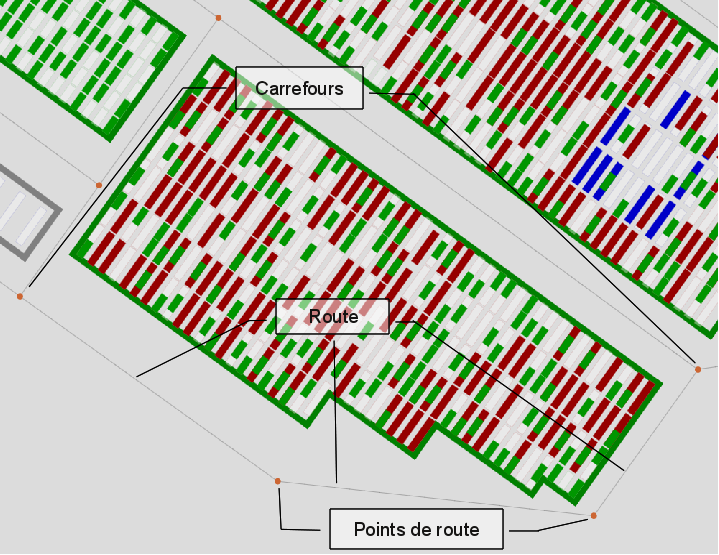
\includegraphics[width=0.6\textwidth]{chapitres/simulation/grapheRoutier.png}
 \caption{Exemple de routes comportant des points de route sur le Terminal de Normandie}
 \label{fig:simulation:grapheRoutier}
\end{figure}

Les travées sont des routes réservées aux chariots cavaliers sur lesquelles ces engins ne peuvent pas se croiser. Une travée est modélisée par un arc First In, First Out (FIFO) relié aux routes par des points de travées. Un point de travée est un point de route reliant à la fois deux arcs et une ou plusieurs travées. Avec cette modélisation il est possible de représenter le réseau routier de n'importe quel terminal à conteneurs.

\subsection{Réseau de stockage}

Avant le début du projet CALAS, le terminal était composé de 2 principaux sous-systèmes. D'une part le réseau routier permettant aux véhicules de se déplacer à l'intérieur du terminal et d'autre part le réseau de stockage. Ce dernier est composé de 3 zones (voir fig. \ref{fig:simulation:3zones}) :
\begin{itemize}
 \item La \textbf{zone maritime} (\textit{Quay side}) permettant de charger ou de décharger la cargaison des navires;
 \item La \textbf{zone de stockage interne} (\textit{Yard}) dédiée au stockage temporaire des conteneurs en attente de transit;
 \item La \textbf{zone terrestre} (\textit{Land side}) permettant de charger ou de décharger la cargaison des véhicules terrestres, c'est-à-dire des camions et des trains.
\end{itemize}

\begin{figure}[h]
 \centering
 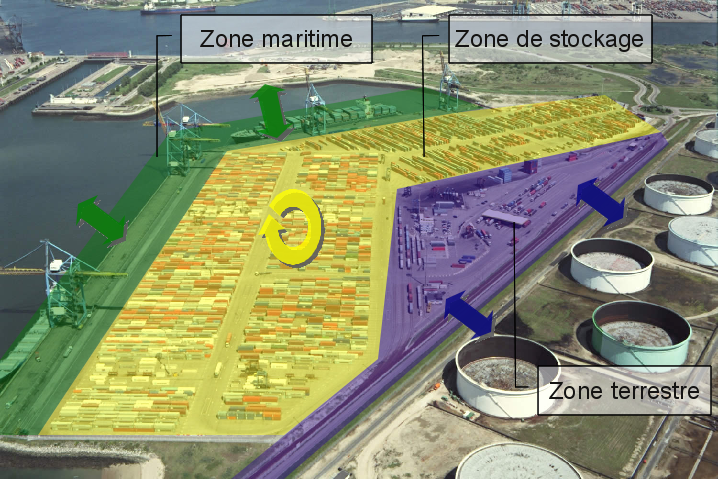
\includegraphics[width=0.6\textwidth]{chapitres/simulation/3zonesDuTN.png}
 \caption{Les 3 types de zones du Terminal de Normandie}
 \label{fig:simulation:3zones}
\end{figure}

Chacune des zones est en interaction avec le réseau routier et comporte différents type d'engins de manutention. Des grues de quai sont utilisées dans la zone maritime pour charger/décharger les navires. Dans le cas d'un déchargement, les conteneurs sont posés sur le quai par la grue puis un chariot cavaliers se charge de transporter le conteneur vers sa destination, c'est-à-dire soit la zone de stockage, soit la zone terrestre, ou soit, dans le cas d'un cabotage, à un autre endroit sur la zone maritime. Dans le cas d'un chargement c'est le chariot cavalier qui amène le conteneur au pied de la grue. Concernant la zone de stockage et la zone terrestre, ce sont les chariots cavaliers qui sont affectés directement au chargement/déchargement des camions ou des trains et au transport des conteneurs entre les zones. Ces véhicules sont capables de transporter un conteneur sur 3 voire 4 niveaux pour les plus récents. Ils peuvent ainsi se déplacer avec un conteneur dans une travée de 3 étages pour les meilleurs et 2 
étages pour les autres.

Chaque zone est composée de pavés. Un pavé (ou bloc) est un regroupement de travées de conteneurs. Chaque pavé comporte donc un certain nombre de travées. Une travée est reliée au réseau routier par des points de travée et représente donc une route particulière qui ne peut être empruntée que par les chariots cavaliers. Elles comportent une série d'emplacements de différentes longueurs pour stocker les conteneurs. Les emplacements où se garent les camions pour être chargés/déchargés sont ainsi modélisés par une travée ne comportant qu'un seul emplacement. Les wagons de trains sont eux aussi modélisés par des travées ne pouvant contenir qu'un seul étage de conteneurs. Pour ces deux types de véhicules, les emplacements sont disponibles si le camion ou le train est en place. Dans le cas contraire, les chariots cavaliers ne peuvent effectuer le chargement ou le déchargement du conteneur.

\subsection{Système de géolocalisation laser (LDTT)}

Suite au projet CALAS, le terminal de Normandie s'est vu doté d'un troisième sous-système : la géolocalisation des engins de manutention. En effet, un réseau de bornes laser a été déployé sur le terminal dans le but de mesurer avec précision la position des véhicules. Ces bornes communiquent avec un serveur central afin de transmettre les coordonnées des chariots. Ce système a été modélisé en simulant la détection des chariots par les bornes selon une certaine portée. Une fois détecté, la borne laser envoie la position du véhicule au système central qui mets à jour les informations connues sur ce chariot. De cette façon, si un véhicule se trouve en dehors de la couverture du réseau de bornes laser, le système ne reproduit que sa dernière position connue. La figure \ref{fig:simulation:laser} montre une la vue 2D du Terminal de Normandie dans le simulateur, et où chaque cercle représente la portée d'une borne laser.

\begin{figure}[h]
 \centering
 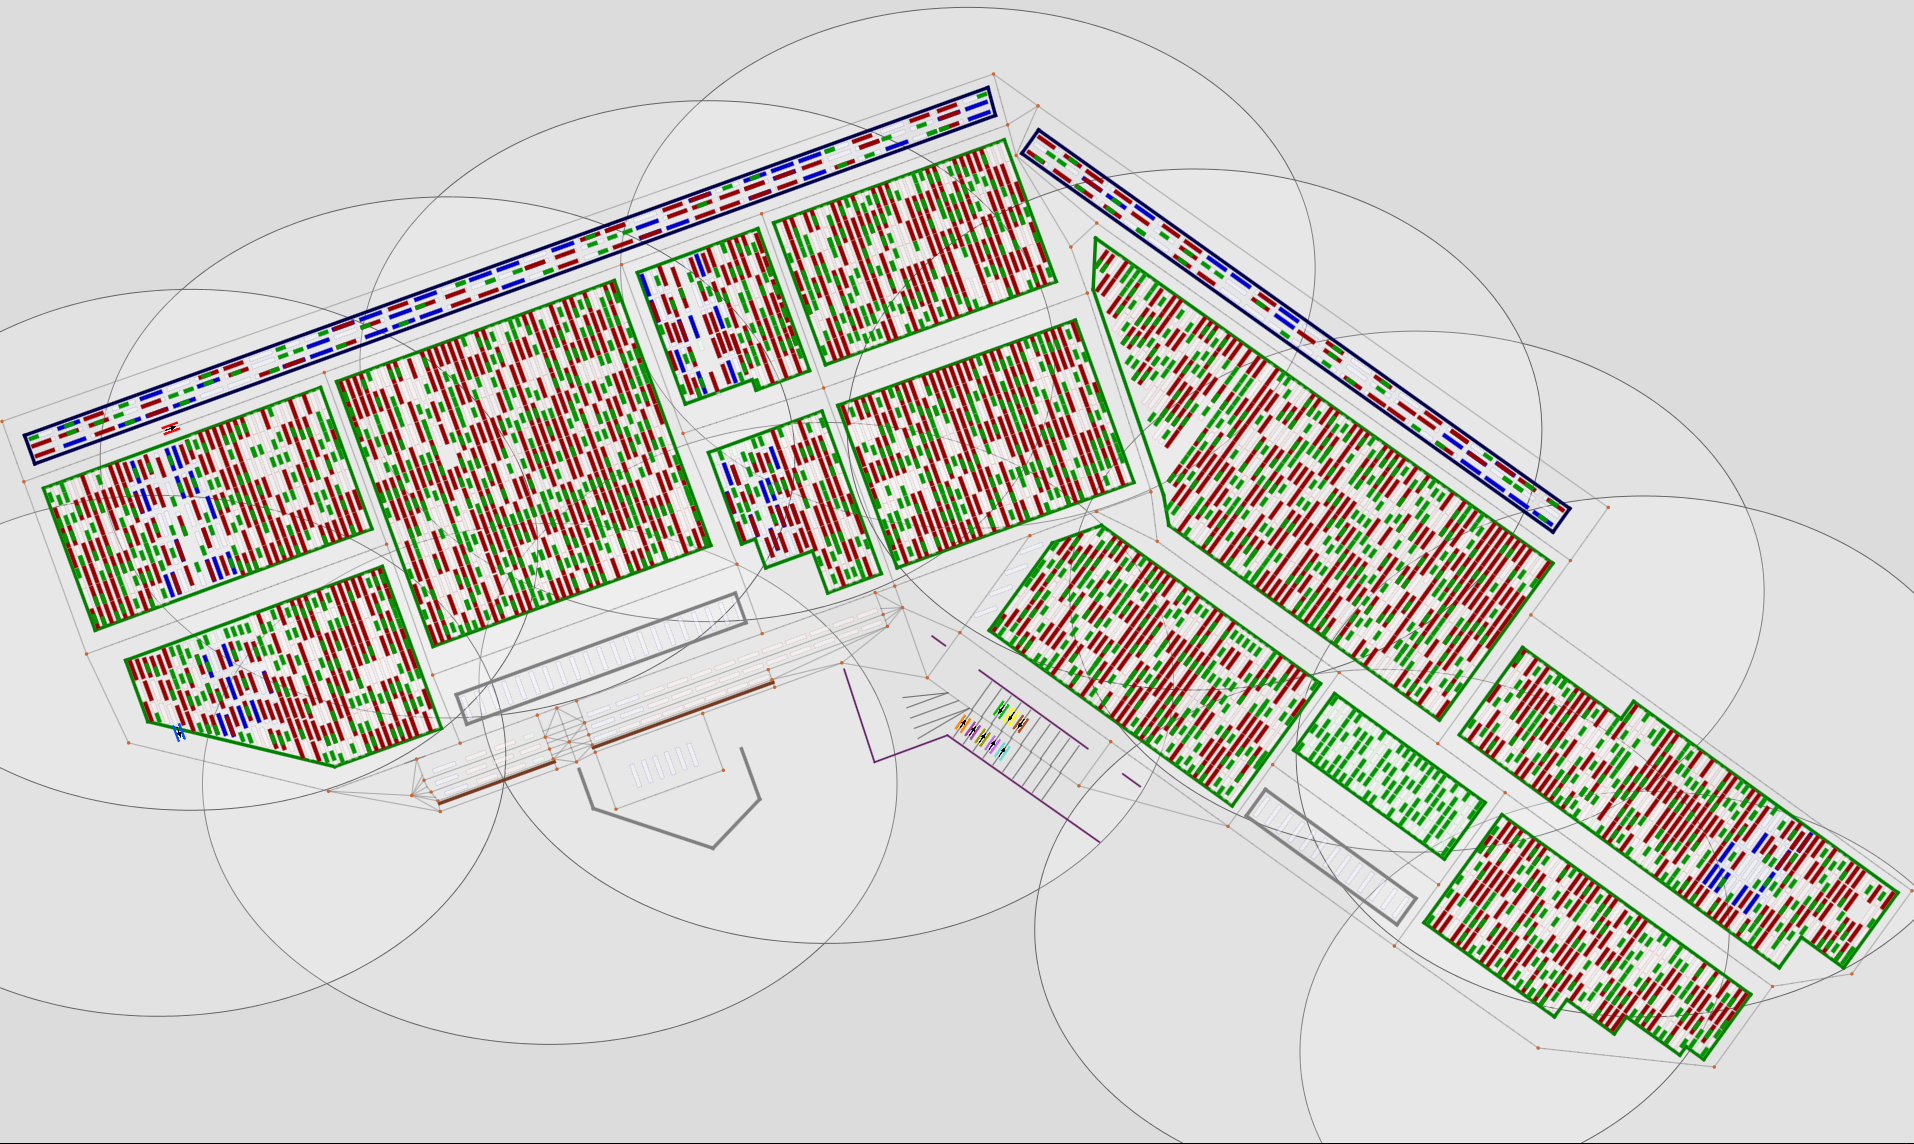
\includegraphics[width=0.8\textwidth]{chapitres/simulation/captureBornesLaser.png}
 \caption{Vue 2D du simulateur montrant le Terminal de Normandie ainsi que le système de localisation laser}
 \label{fig:simulation:laser}
\end{figure}

\subsection{Mobilité au sein du terminal}

Dans la modélisation choisie ici, seuls les chariots cavaliers sont mobiles. En effet, ils sont les seuls véhicules à pouvoir déplacer les conteneurs au sein du terminal. La mobilité des autres véhicules (navires, camions et trains) ne comporte que les actions d'arrivée et de départ. Ainsi, un camion est soit sur son emplacement de chargement/déchargement, soit en dehors du terminal. Toutefois, d'autres véhicules peuvent être ajoutés facilement en décrivant leur comportement dans le
simulateur. 

Les chariots cavaliers sont donc les seuls véhicules à pouvoir emprunter les travées de conteneurs. Cependant, ils ne peuvent pas se croiser à l'intérieur de celles-ci. C'est cet élément qui caractérise les arcs (ou arêtes) de type travée. En effet, les travées sont \textit{First-In-First-Out} (premier entré, premier sorti), c'est-à-dire que les véhicules sortent de la travée dans le même ordre qu'ils y sont entrés. Pour éviter des blocages, les chariots cavaliers n'ont pas l'autorisation d'emprunter une travée déjà occupée par un autre chariot. Si la travée est prise, ils devront attendre à l'entrée de celle-ci jusqu'à ce qu'elle soit libérée.

Sur les routes, les chariots peuvent se croiser et se doubler. Néanmoins, les dépassements ne sont pas modélisés fidèlement, c'est-à-dire que les différentes voies de circulation ne sont pas modélisées et que les collisions ne sont pas prises en compte. Ce procédé permet de simplifier la modélisation sans pour autant dégrader la qualité de la simulation. En effet, suite à une collision, les véhicules deviendront simplement indisponibles (en panne) durant un certain temps.

Le comportement des conducteurs des chariots est complexe à reproduire. En théorie, ces derniers choisissent une mission à effectuer parmi celles que le système leur propose et se rendent sur les emplacements de collecte et de livraison de conteneurs selon l'itinéraire affecté par le système. En réalité les conducteurs s'échangent des missions entres eux et choisissent leur propre itinéraire. Ces comportements ont été modélisés par des événements de non respect d'affectation et d'itinéraire. De cette façon, il est possible d'introduire de la dynamicité dans la simulation et surtout de pouvoir la quantifier facilement.

\subsection{Temporalité}

L'objectif étant d'étudier l'impact de la dynamicité sur l'évolution du système, la modélisation du temps est essentielle. Il a été décidé de se placer dans le cas discret, avec un pas de temps réglable. Ainsi, il est possible de modéliser les événements liés à la dynamique.

Le simulateur permettant de préciser le pas de temps pour une simulation, il sera possible d'étudier l'influence du choix du pas de temps sur les résultats des simulations au niveau macro. La figure \ref{fig:simulation:temporalite} montre deux captures d'écran d'une simulation à 1 pas de temps d'intervalle. Ici le véhicule mauve situé dans le quart inférieur droit de l'image continue son déplacement. La vitesse du véhicule étant de 27km/h, il aura effectué 15 mètres pendant les 2 secondes simulées.

\begin{figure}[h]
  \centering
  \begin{tabular}{c}
    \subfloat[Capture d'écran du simulateur à t=3m33s]{\label{subfig:capture1}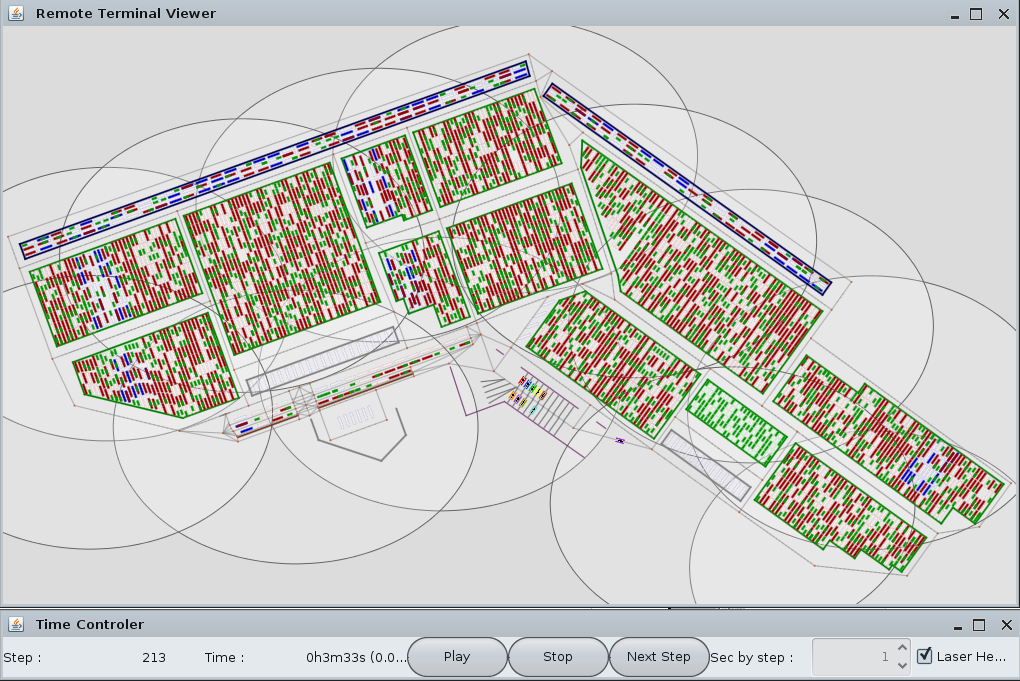
\includegraphics[width=0.9\textwidth]{chapitres/simulation/capture3m33s.png}} \\
    \subfloat[Capture d'écran du simulateur à t=3m35s]{\label{subfig:capture2}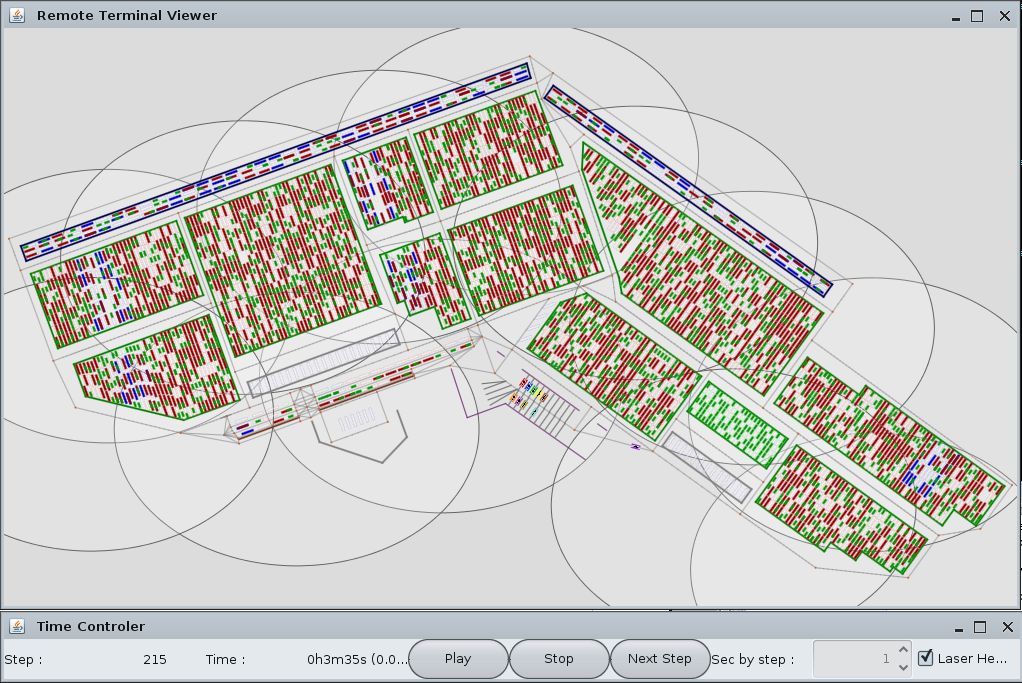
\includegraphics[width=0.9\textwidth]{chapitres/simulation/capture3m35s.png}} \\
  \end{tabular}
  \caption{Exemple de représentation discrète du temps, ici avec un pas de temps de 2 secondes par itération}
  \label{fig:simulation:temporalite}
\end{figure}

\FloatBarrier

\subsection{Événements}

Les événements interviennent au cours du temps et possèdent donc un marqueur temporel de déclenchement. Il existe des événements de différentes natures :
\begin{itemize}
 \item arrivée de mission : une nouvelle mission est connue du système;
 \item annulation de mission : une mission déjà connue est retirée du système;
 \item arrivée de véhicule (bateau, camion, train) : un véhicule est arrivé sur son/ses emplacements;
 \item départ de véhicule (bateau, camion, train) : un véhicule a quitté son/ses emplacements;
 \item panne de chariot cavalier : un chariot est indisponible;
 \item fin de panne de chariot cavalier : un chariot indisponible redevient disponible;
 \item non respect d'affectation de mission d'un chariot cavalier : le conducteur d'un chariot a choisi une mission qui ne lui était pas destinée;
 \item non respect d'itinéraire d'un chariot cavalier : le conducteur d'un chariot a choisi un itinéraire différent de celui proposé par le système;
 \item perte de conteneur : un conteneur ne se trouve pas à l'emplacement indiqué par le système.
\end{itemize}

L'objectif est de reproduire un terminal portuaire à conteneurs tant dans son contenu que dans son comportement. Chaque sous-système du terminal a donc été modélisé ainsi que les interactions, à la fois à l'intérieur et entre ces sous-systèmes.
 
\section{Collecte des données}

Une fois le modèle établi, il est nécessaire de collecter des données afin de décrire un terminal existant. Le choix s'est porté sur le Terminal de Normandie, un des terminaux du Port Autonome du Havre directement impliqué dans le projet CALAS.

La difficulté rencontrée quant à l'obtention d'information concernant les données du terminal est l'une des raisons pour lesquelles le développement d'un simulateur a été la solution retenue pour de mettre au point et tester la performance de nos méthodes. Une grande partie du temps alloué au projet a donc été consacré à la collecte d'informations sur : 
\begin{itemize}
 \item Les chariots cavaliers : dimensions, vitesse, comportement;
 \item Le fonctionnement du terminal : différentes zones d'échange, zone de stockage, engins de manutention;
 \item Le réseau routier du terminal : 
  \begin{itemize}
   \item coordonnées des carrefours;
   \item routes;
   \item travées;
   \item coordonnées des emplacements conteneurs dans les travées;
   \item zone de dépôt des engins de manutention.
  \end{itemize}
\end{itemize}

Les coordonnées des carrefours, routes, travées et emplacements conteneurs du Terminal de Normandie ont été obtenus grâce à un plan sommaire du terminal fourni par nos partenaires du projet CALAS (voir figure \ref{fig:planTerminalSommaire}) et au site internet de cartographie \href{http://wikimapia.org/\#lat=49.4694697\&lon=0.1676486\&z=16\&l=2\&m=b}{wikimapia.org}. Ce site permet de mesurer de façon relativement précise des distances sur des photos satellites d'une grande définition. Les coordonnées indiquées sur le plan fourni par nos partenaires sont exprimés en suivant la projection conique conforme de Lambert (zone centre : Lambert II). Un degré de ce système correspond à 100km. Cette équivalence permet de calculer aisément les coordonnées des points manquant du plan grâce aux distances mesurées sur le site \href{http://wikimapia.org/\#lat=49.4694697\&lon=0.1676486\&z=16\&l=2\&m=b}{wikimapia.org}.

\begin{figure}[ht]
\centering
 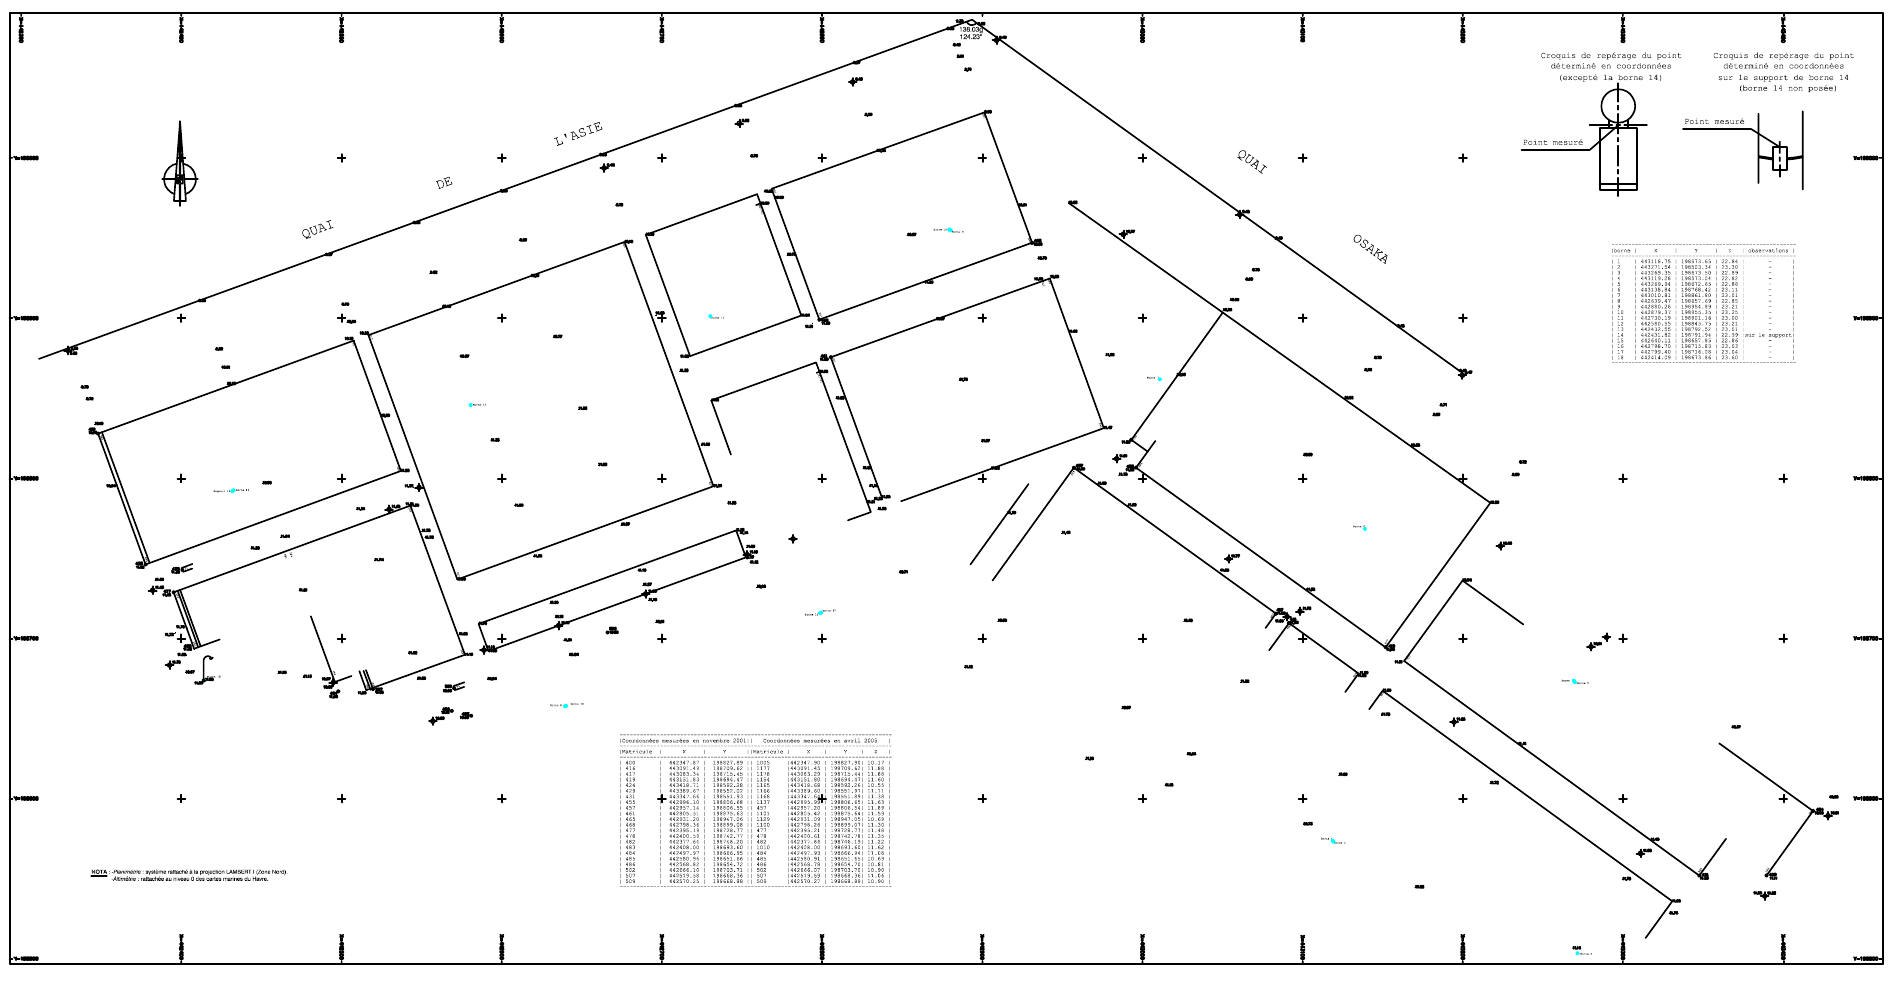
\includegraphics[width=0.8\textwidth]{./chapitres/simulation/planTerminalSommaire.png}
  \caption{Plan sommaire du Terminal de Normandie}
  \label{fig:planTerminalSommaire}
\end{figure}

La figure \ref{fig:planTerminalComplet} montre le plan obtenu grâce aux recroisemment des informations du plan sommaire et de \href{http://wikimapia.org/\#lat=49.4694697\&lon=0.1676486\&z=16\&l=2\&m=b}{wikimapia.org}. Le Terminal de Normandie, loin d'être le plus grand au monde, comporte tout de même 1170 carrefours, 170 routes, 531 travées et 3499 emplacements conteneurs.

\begin{figure}[ht]
\centering
 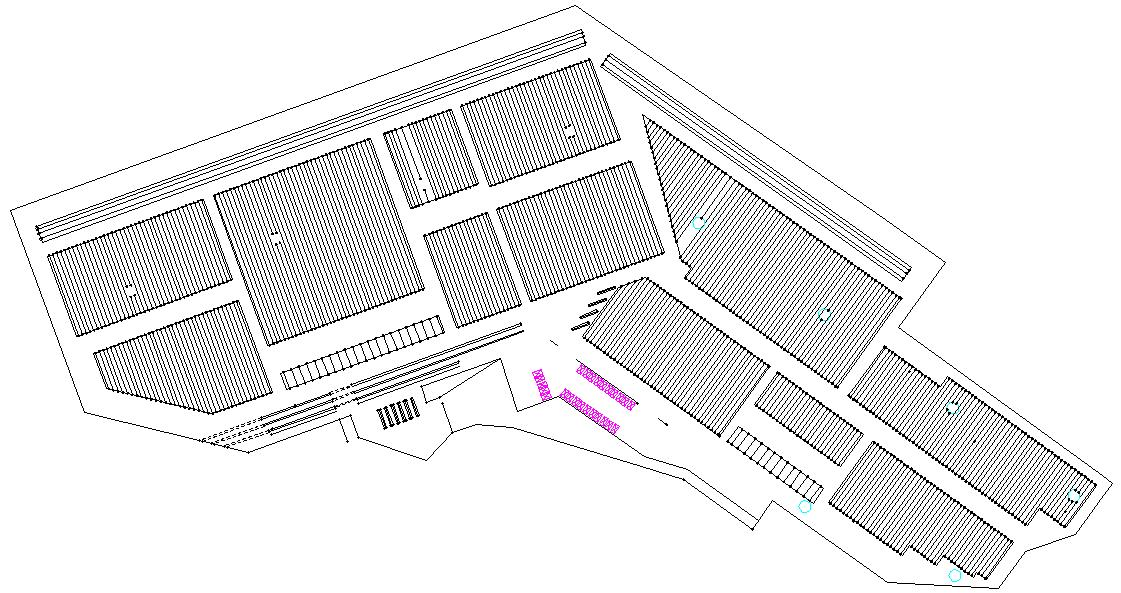
\includegraphics[width=0.8\textwidth]{./chapitres/simulation/planTerminalComplet.jpg}
  \caption{Plan du Terminal de Normandie obtenu après collecte et recoupement des données}
  \label{fig:planTerminalComplet}
\end{figure}

D'autre part, les images satellites ont également permis de collecter des données sur les chariots cavaliers et notamment leur lieu de stationnement (dépôt). Des données concernant les chariots
cavaliers ont également été récupérées sur les sites des constructeurs afin de connaître leurs principales dimensions :
\begin{itemize}
 \item longueur hors tout ;
 \item largeur hors tout ;
 \item hauteur hors tout ;
 \item longueur des panneaux latéraux ;
 \item largeur interne (entre les deux panneaux latéraux) ;
\end{itemize}

ainsi que des informations sur la vitesse moyenne de fonctionnement, les temps de manutention, etc. Toutes ces informations sont décrites dans des fichiers au format \verb!XML!.

\section{Structuration des données}\label{sec:structurationDonnees}

Les données des simulations sont décrites dans des fichiers \verb!XML!. L'Extensible Markup Language (langage extensible de balisage 5) permet de définir de façon lisible des caractéristiques et des comportements dans de simple fichiers texte et sont également rapidement interprétables par le programme. Il existe différents fichiers de configurations nécessaires au fonctionnement du simulateur :
\begin{itemize}
 \item le fichier de déploiement de l'application;
 \item le fichier de configuration du système de localisation laser (position et portée des bornes);
 \item le fichier de description des véhicules;
 \item le fichier de configuration du terminal (zones de stockage, réseau routier);
 \item le fichier d'initialisation du terminal permettant de décrire la position des conteneurs au démarrage de la simulation;
 \item les fichiers d'événements (missions, pannes de véhicule ou de borne laser, arrivées ou départs des véhicules clients, etc).
\end{itemize}

\subsection{Réseau routier}\label{sec:description:resRoutier}

Les routes et les carrefours d'un terminal portuaire à conteneurs constituent un graphe. Ainsi, les n\oe{}uds du graphe sont des carrefours et les routes sont des arcs. La structure \verb!XML! doit donc permettre de décrire ce graphe. Les coordonnées sont exprimées en mètres selon la projection conique de Lambert.

\begin{figure}[h]
 
\begin{lstlisting}[language=XML]
  <crossroad id='' x='' y=''/>
  <road
    id=''
    origin='crossroadId'
    destination='crossroadId'
    [directed='boolean']
  />
\end{lstlisting}
\caption{Code XML nécessaire à la description d'un carrefour et d'une route}
\label{fig:simulation:carrefourRoute}
\end{figure}

Un arc étant représenté par une droite entre deux n\oe{}uds, l'objet roadpoint (point de route) a été introduit pour permettre de modéliser des routes sinueuses. Ainsi une route est une liste d'arcs dont le premier part d'un n\oe{}ud et le dernier se termine par un autre n\oe{}ud. Tous les autres arcs de cette route relient des points de route. La figure \ref{fig:simulation:ptsRoute} donne un exemple de code \verb!XML! décrivant une route reliant le carrefours A au carrefour B et utilisant deux points de route, ainsi que le graphe ainsi généré.

\begin{figure}[h]
 
\begin{lstlisting}[language=XML]
<crossroad id='A' x='0' y='1' > </crossroad>
<crossroad id='B' x='3' y='1' > </crossroad>
<road id=' ' origin='A' destination='B'>
<roadpoint id='C' x='1' y='2' > premier point </roadpoint>
  <!--... autres points de route eventuels -->
<roadpoint id='D' x='2' y='0' > dernier point </roadpoint>
</road>
\end{lstlisting}

{
\centering
\tikzstyle{vertex}=[circle,draw,fill=white,line width=0.5pt,minimum size=25pt,inner sep=0pt,font=\tiny]
\tikzstyle{edge} = [draw,thick,->]
 \begin{tikzpicture}[xscale=3, yscale=0.5, auto,swap]
     \foreach \pos/\name in {
	{(0,1)/A},
	{(3,1)/B}, {(1,2)/C},
	{(2,0)/D}}
      \node[vertex] (\name) at \pos {$\name$};

    \foreach \source/ \dest in {A/C, C/D, D/B} \path[edge] (\source) node[] {} -- node[] {} (\dest);
\end{tikzpicture}\\
}
\caption{Exemple de description XML d'un arc comportant des points de route}
\label{fig:simulation:ptsRoute}
\end{figure}

\subsection{Zones de stockage}\label{sec:description:zonesStockage}

Il existe deux types de zones sur un terminal à conteneurs. D'une part, les zones d'échanges (quais, zone ferroviaire et zone routière) et les zones de stockage d'autre part. Une zone est modélisée par la balise \verb!<pave id='' type='{BOAT, ROAD, TRAIN, STOCK}'>! \verb!</pave>!. À l'intérieur de cette balise se trouvent les coordonnées des contours de la zone. La balise \verb!<wall from='' to=''>! \verb!</wall>! permet de relier ces points.

\begin{subfigures}
\begin{figure}
\centering
 \begin{lstlisting}[language=XML]
<pave id="L" type="ROAD">
<coordinate id="L-NW" x="443051.6250" y="198654.4978"/>
<coordinate id="L-NE" x="443138.2976" y="198591.7532"/>
<coordinate id="L-SE" x="443127.3772" y="198576.6273"/>
<coordinate id="L-SW" x="443040.6241" y="198639.2604"/>
<wall from="L-NW" to="L-NE"/>
<wall from="L-NE" to="L-SE"/>
<wall from="L-SE" to="L-SW"/>
<wall from="L-SW" to="L-NW"/>
</pave>
\end{lstlisting}
\caption{Code XML d'une zone de chargement/déchargement de camions}
\end{figure}

\begin{figure}[h]
  \centering
  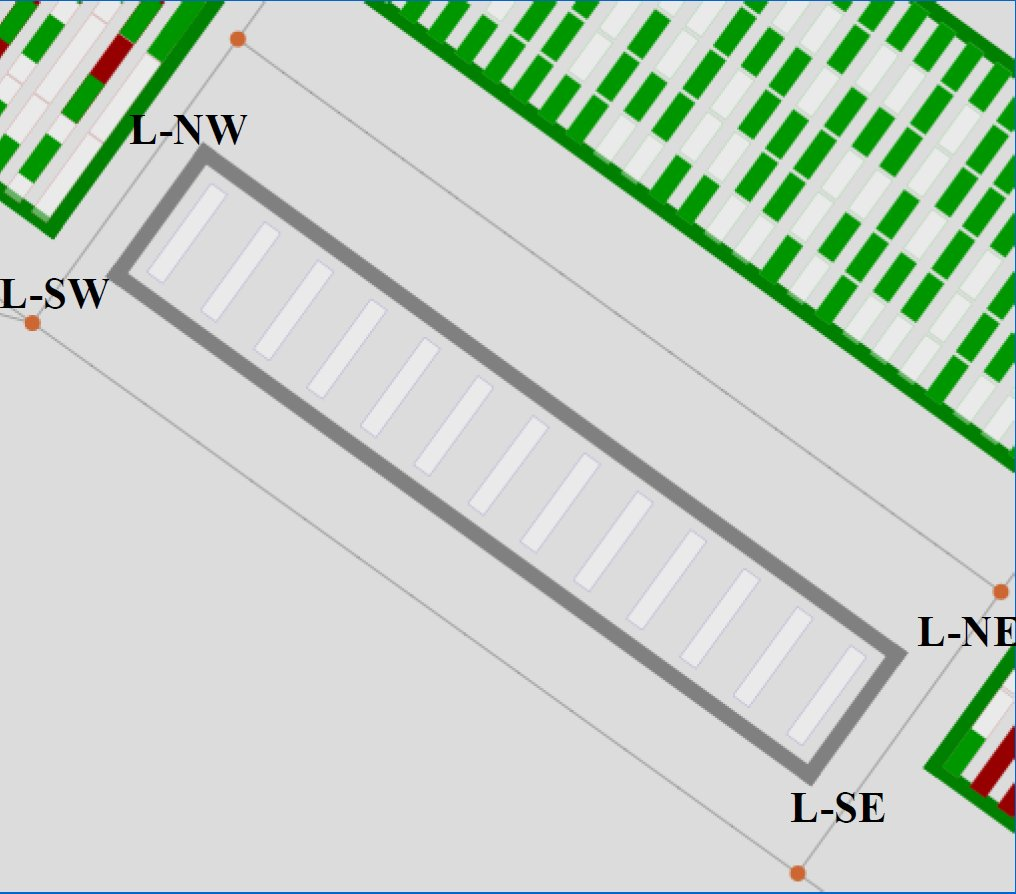
\includegraphics[width=0.75\textwidth]{chapitres/simulation/pave.jpg}
  \caption{Rendu 2D de cette zone dans $D^2CTS$ }
\end{figure}
\label{fig:simulation:pave}
\end{subfigures}

Les travées sont également décrites à l'intérieur de la balise \verb!<pave>! de la zone concernée. Les points d'entrée et de sortie des travées sur les routes sont des points de routes spécifiques décrits par la balise \verb!<laneCrossroad>! et sont insérés à l'intérieur de la balise \verb!<road>! de la route permettant d'accéder à la travée.
La balise \verb!<lane id='' origin='' destination='' slots=''>! permet de décrire une travée grâce à l'identifiant, le point d'entrée, le point de sortie et la description des emplacements conteneurs de cette travée. Cette dernière information est donnée sous la forme : $tailleConteneurEnPieds*nombreD'emplacementsDeCetteTaille$

Par exemple, une travée comportant 2 emplacements de 40 pieds puis 1 emplacement de 20 pieds sera décrite en \verb!XML! de la façon suivante :
\begin{lstlisting}[language=XML]
<lane id='' origin='' destination='' slots='40*2-20*1'/>
\end{lstlisting}

De plus, les coordonnées du premier et du dernier emplacement de la travée peuvent être précisées grâce aux paramètres \verb!in='coordX,coordY'! et \verb!out='coordX,coordY'!. Dans le cas contraire, ces coordonnées sont calculées de façon à conserver la même distance entre les conteneurs ainsi qu'entre le premier emplacement et le point d'entrée de la travée et entre le dernier emplacement et le point de sortie de la travée. Si les coordonnées \verb!in! et \verb!out! sont précisées alors les emplacements contenus entre le premier et le dernier sont répartis de façon régulière entre ces deux emplacements. 
Les emplacements de trains et de camions sont modélisés par des travées spécifiques. Ces travées sont décrites par la balise \verb!<exchangeLane>! en \verb!XML!. Les paramètres sont les mêmes que pour une travée classique (\verb!<lane>!). La figure \ref{fig:simulation:travee} donne un exemple d'utilisation de ces balises.

\begin{figure}[ht]
\centering
 \begin{lstlisting}[language=XML]
<pave id="L" type="ROAD">
<coordinate id="L-NW" x="443051.6250" y="198654.4978"/>
<coordinate id="L-NE" x="443138.2976" y="198591.7532"/>
<coordinate id="L-SE" x="443127.3772" y="198576.6273"/>
<coordinate id="L-SW" x="443040.6241" y="198639.2604"/>
<wall from="L-NW" to="L-NE"/>
<wall from="L-NE" to="L-SE"/>
<wall from="L-SE" to="L-SW"/>
<wall from="L-SW" to="L-NW"/>
<road id="c32-c38" origin="c32" destination="c38">
<laneCrossroad id="L_S_1" x="443037.4695" y="198627.9259"/>
<laneCrossroad id="L_S_2" x="443044.1513" y="198623.1196"/>
<laneCrossroad id="L_S_3" x="443050.8331" y="198618.3134"/>
<laneCrossroad id="L_S_4" x="443057.5149" y="198613.5071"/>
<laneCrossroad id="L_S_5" x="443064.1967" y="198608.7009"/>
<laneCrossroad id="L_S_6" x="443070.8785" y="198603.8946"/>
<laneCrossroad id="L_S_7" x="443077.5602" y="198599.0884"/>
<laneCrossroad id="L_S_8" x="443084.2420" y="198594.2822"/>
<laneCrossroad id="L_S_9" x="443090.9238" y="198589.4759"/>
<laneCrossroad id="L_S_10" x="443097.6056" y="198584.6697"/>
<laneCrossroad id="L_S_11" x="443104.2874" y="198579.8634"/>
<laneCrossroad id="L_S_12" x="443110.9692" y="198575.0572"/>
<laneCrossroad id="L_S_13" x="443117.6509" y="198570.2510"/>
</road>
<exchangeLane id="L-1/13" origin="L_N_1" destination="L_S_1" slots="45*1" in="443054.9578,198652.0845" out="443043.9608,198636.8514"/>
<exchangeLane id="L-2/13" origin="L_N_2" destination="L_S_2" slots="45*1" in="443061.6258,198647.2580" out="443050.6341,198632.0335"/>
<exchangeLane id="L-3/13" origin="L_N_3" destination="L_S_3" slots="45*1" in="443068.2929,198642.4315" out="443057.3074,198627.2155"/>
<exchangeLane id="L-4/13" origin="L_N_4" destination="L_S_4" slots="45*1" in="443074.9600,198637.6050" out="443063.9807,198622.3976"/>
<exchangeLane id="L-5/13" origin="L_N_5" destination="L_S_5" slots="45*1" in="443081.6271,198632.7785" out="443070.6540,198617.5797"/>
<exchangeLane id="L-6/13" origin="L_N_6" destination="L_S_6" slots="45*1" in="443088.2942,198627.9520" out="443077.3273,198612.7617"/>
<exchangeLane id="L-7/13" origin="L_N_7" destination="L_S_7" slots="45*1" in="443094.9613,198623.1255" out="443084.0007,198607.9438"/>
<exchangeLane id="L-8/13" origin="L_N_8" destination="L_S_8" slots="45*1" in="443101.6284,198618.2990" out="443090.6740,198603.1259"/>
<exchangeLane id="L-9/13" origin="L_N_9" destination="L_S_9" slots="45*1" in="443108.2956,198613.4724" out="443097.3473,198598.3080"/>
<exchangeLane id="L-10/13" origin="L_N_10" destination="L_S_10" slots="45*1" in="443114.9627,198608.6459" out="443104.0206,198593.4900"/>
<exchangeLane id="L-11/13" origin="L_N_11" destination="L_S_11" slots="45*1" in="443121.6298,198603.8194" out="443110.6939,198588.6721"/>
<exchangeLane id="L-12/13" origin="L_N_12" destination="L_S_12" slots="45*1" in="443128.2969,198598.9929" out="443117.3672,198583.8542"/>
<exchangeLane id="L-13/13" origin="L_N_13" destination="L_S_13" slots="45*1" in="443134.9640,198594.1664" out="443124.0405,198579.0362"/>
</pave>
\end{lstlisting}
\caption{Exemple de code XML de description d'une travée}
\label{fig:simulation:travee}
\end{figure}

\FloatBarrier

\subsection{Conteneurs}

Le simulateur tient compte de l'hypothèse selon laquelle il existe 3 types de conteneurs sur le Terminal de Normandie. D'abord les conteneurs de 20 pieds : 1 TEU (twenty feet equivalent unit); les conteneurs de 40 pieds : 2 TEU ; et enfin les conteneurs de 45 pieds : 2.25 TEU qui sont des conteneurs réfrigérés. Les dimensions de ces conteneurs sont les suivantes (normes ISO) :

\begin{center}
\footnotesize
\begin{tabular}{|c|c|c|c|}
  \hline
  \textbf{\textit{Type}} & \textbf{\textit{Longueur (m)}} & \textbf{\textit{Largeur (m)}} & \textbf{\textit{Hauteur (m)}} \tabularnewline
  \hline
  20 pieds & 6,058 & 2,438 & 2,591 \tabularnewline
  \hline
  40 pieds & 12,192 & 2,438 & 2,591 \tabularnewline
  \hline
  45 pieds & 13,716 & 2,438 & 2,896 \tabularnewline
  \hline
\end{tabular}
\end{center}

Pour pouvoir décrire un conteneur en \verb!XML! il faut donner l'identifiant du conteneur et son type (en TEU). Il est également possible de spécifier sa position. Cette dernière est définie par un pavé, une travée, un emplacement, un niveau et enfin un alignement. 
Le niveau correspond à l'étage auquel le conteneur est stocké sur l'emplacement. L'étage 0 correspond au rez-de-chaussé (le conteneur est posé sur le sol du terminal). Il est possible de stocker deux niveaux de conteneurs dans les travées de stockage et un seul niveau sur les trains et les camions.
L'alignement du conteneur permet de définir si le conteneur est centré sur son emplacement, c'est-à-dire que l'espace entre les extrémités de l'emplacement et le conteneur est le même, ou si le conteneur est aligné sur un coté de l'emplacement. La valeur \verb!'origin'! correspond à un alignement le plus proche du point d'entrée de la travée de l'emplacement. La valeur \verb!'destination'! correspond quant à elle à l'alignement le plus proche du point de sortie de la travée contenant l'emplacement de stockage.

\begin{figure}[ht]
\centering
 \begin{lstlisting}[language=XML]
<container id="LWCU 429852 1" teu="2.25">
  <containerLocation pave="Asie" lane="Asie-3/3" slot="Asie-3/3-34" level="0" align="center"/>
</container>
\end{lstlisting}
\caption{Exemple de code XML de description d'un conteneur}
\label{fig:simulation:conteneur}
\end{figure}

\subsection{Missions}

Une mission est un déplacement de conteneur au sein du terminal. Elle comporte 2 phases. Tout d'abord la phase de collecte du conteneur par le chariot cavalier, c'est la phase de \textit{pickup}. Dans cette phase le chariot effectue le trajet de son point de départ vers la position courante du conteneur. Il doit respecter une fenêtre de temps pour pouvoir le récupérer. Une fois le chariot en position et le conteneur récupéré, la deuxième phase, celle de livraison du conteneur (\textit{delivery}) commence. Cette phase consiste à amener le conteneur sur son emplacement de destination, tout en respectant également une fenêtre de temps. Une fois la destination atteinte, le conteneur est déchargé du chariot et déposé sur son emplacement de destination. La mission est alors terminée. Pour pouvoir décrire ces différentes opérations la structure \verb!XML! de la balise \verb!<mission>! se compose d'un identifiant, de l'identifiant du conteneur concerné et du type de mission. Une mission peut être de type :
\begin{itemize}
 \item STAY : un conteneur doit être déplacé d'une zone de stockage du terminal à une autre et donc va rester dans le terminal ;
 \item IN : un conteneur provenant d'un véhicule externe (train, camion ou bateau) doit être déplacé dans une zone de stockage du terminal et donc va entrer dans le terminal ;
 \item OUT : un conteneur d'une zone de stockage doit être chargé sur un véhicule extérieur (train, camion ou bateau) et donc va sortir du terminal ;
 \item IN\_AND\_OUT : un conteneur doit être déchargé d'un véhicule externe puis être chargé sur un autre véhicule externe. Dans ce type de mission, le conteneur ne passe pas par une zone de stockage.
\end{itemize}

Chaque type comporte un identifiant numérique :

\begin{center}
\footnotesize
\begin{tabular}{|c|c|}
  \hline
  \textbf{\textit{Type}} & \textbf{\textit{Identifiant}}\tabularnewline
  \hline
  STAY & 0 \tabularnewline
  \hline
  IN & 1 \tabularnewline
  \hline
  OUT & 2 \tabularnewline
  \hline
  IN\_AND\_OUT & 3 \tabularnewline
  \hline
\end{tabular}
\end{center}

Il est possible de spécifier dans le paramètre \verb!'kind'! de la balise \verb!<mission>! soit le type de mission, soit son identifiant. Une fois ces trois paramètres fournis, il faut définir les fenêtres de temps de collecte (\textit{pickup}) et de livraison (\textit{delivery}) et l'emplacement de destination du conteneur. La balise \verb!<timewindow>! correspond à la description d'une fenêtre de temps et comporte les paramètres \verb!start! et \verb!end! correspondant respectivement à l'heure de début et de fin de cette fenêtre de temps. Le temps est donné sous la forme \verb!hh:mm:ss.ms!. La destination du conteneur pour la mission est définie par la balise \verb!<containerLocation>! décrite précédemment.

\begin{figure}[ht]
\centering
 \begin{lstlisting}[language=XML]
<mission id="m24" container="TXIU 696005 5" kind="0">
  <timewindow start="00:10:39.49" end="00:15:59.24"/>
  <timewindow start="00:12:05.23" end="00:18:07.85"/>
  <containerLocation pave="N" lane="N-25/42" slot="N-25/42-0" level="1" align="center"/>
</mission>
\end{lstlisting}
\caption{Exemple de code XML de description d'une mission}
\label{fig:simulation:mission}
\end{figure}

\subsection{Bornes de positionnement laser}\label{sec:description:bornesLaser}

Le système de géolocalisation laser doit être décrit dans un fichier indépendant. Dans ce fichier la description du système comportera plusieurs informations. Une borne a un identifiant (\verb!'id'!), une position (\verb!'x'!, \verb!'y'! et \verb!'z'!) et une portée (\verb!'rangeX'!, \verb!'rangeY'! et \verb!'rangeZ'!) indiquée en mètres.

\begin{figure}[ht]
\centering
 \begin{lstlisting}[language=XML]
<laserheads>
  <laserhead id="1" x="443118.75" y="198573.65" z="22.84" rangeX="125" rangeY="100" rangeZ="40"/>
  <laserhead id="2" x="443271.54" y="198503.34" z="23.30" rangeX="125" rangeY="100" rangeZ="40"/>
</laserheads>
\end{lstlisting}
\caption{Exemple de code XML de description d'un réseau composé de deux bornes laser}
\label{fig:simulation:xmlbornes}
\end{figure}

Si un véhicule se trouve à portée de la borne, alors celle-ci va capter son signal et renvoyer la position au simulateur.

\subsection{Description des véhicules}\label{sec:description:vehicules}

Les informations permettant de décrire les types de chariots cavaliers présents sur le terminal ainsi que les instances de ces types doivent être regroupées dans un fichier. Il est nécessaire de décrire les types (ou modèles de chariots), puis chacun des véhicules.

\subsubsection{Types de chariots cavaliers}

Un type de chariot cavalier donne les informations permettant de décrire les attributs d'un chariot de ce modèle. Il comporte :
\begin{itemize}
\item un identifiant ;
\item la largeur (\verb!'width'!) en mètres ;
\item la hauteur (\verb!'height'!) en mètres ;
\item la longueur (\verb!'length'!) en mètres ;
\item la largeur intérieure (\verb!'innerWidth'!) en mètres correspondant à l'espace libre entre les roues gauches et les roues droites du chariot ;
\item la longueur intérieure (\verb!'innerLength'!) en mètres correspond à la longueur entre les deux barres transversales du chariot ;
\item les longueurs entre ces barres transversales et les extrémités du chariot (\verb!'backOverLength'! et \verb!'frontOverLength'!) en mètres ;
\item la largeur de la cabine (\verb!'cabWidth'!) en mètres ;
\item la vitesse du chariot (\verb!'speed'!) en mètres par seconde ;
\item la vitesse en marche arrière (\verb!'reverseSpeed'!) en mètres par seconde ;
\item la vitesse en travée (\verb!'laneSpeed'!) en mètres par seconde ;
\item la vitesse de demi-tour du poste de pilotage (\verb!'turnBackTime'!) en secondes ;
\item la compatibilité du chariot avec les conteneurs (\verb!'compatibility'!). Cette dernière est décrite de façon binaire. Le premier bit, bit de poids fort, correspond aux conteneurs de 20 pieds, le second aux conteneurs de 40 pieds, et enfin le troisième représente les conteneurs de 45 pieds. Un chariot compatible avec les conteneurs de 40 pieds uniquement aura comme paramètre de compatibilité la valeur \verb!'010'!. Dans le cas d'un chariot compatible avec tous les conteneurs (bras de levage réglable), il est possible de spécifier soit la valeur \verb!'111'! soit la valeur \verb!'all'!.
\end{itemize}

\begin{figure}[ht]
\centering
 \begin{lstlisting}[language=XML]
<type
  id="standard"
  width="5"
  height="15.4"
  length="10"
  innerWidth="3"
  innerLength="6"
  backOverLength="1"
  frontOverLength="3"
  cabWidth="2"
  speed="8.33"
  reverseSpeed="8.33"
  laneSpeed="5"
  turnBackTime="4"
  compatibility="all"
/>
\end{lstlisting}
\caption{Exemple de code XML de description d'un type de chariot cavalier}
\label{fig:simulation:typeChariot}
\end{figure}

\subsubsection{Instances de chariots cavaliers}

Une fois que les modèles de chariots ont été décrit, il est possible de donner la description de chaque chariot. Un chariot possède un identifiant, un type, un emplacement de stationnement dans le dépôt, une couleur, une machine pour la distribution, une route de départ, une position sur cette route sous forme de taux (entre 0 et 1, où 0 est le point d'origine de l'arc et 1 est le point de destination de l'arc), une direction sur cette route sous forme d'un booléen (\verb!true! signifie que le chariot se dirige dans le sens de l'arc, vers le point de destination). Le routage du chariot cavalier est indiqué dans la balise \verb!<routing>! à l'intérieur de la balise du chariot. Il est nécessaire de spécifier le type du routage et la machine qui devra se charger des calculs (\verb!host!).


\begin{figure}[ht]
\centering
 \begin{lstlisting}[language=XML]
<straddleCarrier id="cav1" type="standard" slot="Central_1" color="red" host="localhost" locationRoad="c2-c5" locationPourcent="0.5" direction="true">
  <routing type="RDijkstra" host="localhost"/>
</straddleCarrier>
<straddleCarrier id="cav2" type="standard" slot="Central_2" color="blue" host="localhost" locationRoad="B-4/38" locationPourcent="0.8" direction="true">
  <routing type="RDijkstra" host="localhost"/>
</straddleCarrier>
\end{lstlisting}
\caption{Exemple de code XML de description de deux chariots cavaliers}
\label{fig:simulation:chariot}
\end{figure}

\subsection{Description de l'ordonnanceur de missions}\label{sec:description:ordonnanceur}

L'optimisation de l'affectation et de l'ordonnancement des missions est l'un des objectifs de la participation du LITIS au projet CALAS. Le simulateur à été conçu de manière à permettre l'utilisation de diverses politiques et algorithmes d'ordonnancement et nottament ceux évoqués dans le chapitre précédent (voir \ref{chapitre:ordo} p\pageref{chapitre:ordo}).

La classe abstraite \verb!MissionScheduler! donne la signature des méthodes \verb!precompute()!, \verb!compute()!, et \verb!apply()!. La méthode \verb!precompute()! est appelée par le contrôleur temporel avant l'exécution  d'une itération de la simulation. Puis la méthode \verb!compute()! contient le code d'une itération de l'algorithme d'ordonnancement et doit être appelée à l'intérieur de la méthode \verb!precompute()!. Enfin, la méthode \verb!apply()! est exécutée à la fin de chaque itération de la simulation.
Le principe est que chaque objet puisse effectuer ses calculs sur les mêmes données, puis les résultats sont mis en application quand tous les calculs sont terminés.

La classe abstraite contient également toutes les structures de données nécessaire à l'élaboration de l'ordonnancement (liste des ressources et des tâches) ainsi que des files d'événements.
Les structures concernant les événements concernent : 
\begin{itemize}
 \item les missions et les véhicules à ajouter dans l'ordonnanceur;
 \item les missions et les véhicules à supprimer de l'ordonnanceur;
 \item les missions et les véhicules à mettre à jour (fenêtre de temps, position, vitesse, etc).
\end{itemize}

Chaque accès en écriture sur ces structures déclenche la prise en compte de leur contenu lors de l'exécution de la méthode \verb!precompute()! à l'itération suivante.

D'autre part, les paramètres de la fonction d'évaluation ($F_1'$, $F_2'$, $F_3'$) d'un ordonnancement doit également être défini dans la classe \verb!MissionScheduler!. En revanche, les autres paramètres dépendent de l'implémentation de l'algorithme et seront donc définis dans les classes filles.

Chaque algorithme d'ordonnancement sera donc modélisé par une classe héritant de \newline\verb!MissionScheduler! et contenant la définition des méthodes abstraites. L'implémentation est donc simplifiée au maximum.
Chaque classe fille devra contenir un identifiant unique indiqué dans la variable \verb!rmiBindingName! permettant au \textit{parser} \verb!XML! de déterminer quel algorithme instancier.

Il est donc impératif de modifier le code du \textit{parser} \verb!XML! lors de l'ajout d'un algorithme. Cette modification concerne la classe \verb!util.parser.XMLNetworkConfigurationParser! et plus particulièrement la méthode \verb!startElement(String uri,! \verb!String localName,! \verb!String qName,! \verb!Attributes atts)!. Il est nécessaire d'ajouter le nouveau type à prendre en compte ainsi que les paramètres de l'algorithme. Les modules d'ordonnancement développés avec le simulateur permettront au développeur de réaliser facilement les modifications nécessaires.

\subsection{Événements}

Le simulateur a pour objectif de modéliser un terminal portuaire à conteneurs dans son ensemble : sa structure (réseau routier, zones de stockages, composants...) et également sa dynamique (arrivée de véhicules, de missions, pannes de chariots cavaliers...). Pour cela la balise \verb!<event>! permet de définir une heure de prise en compte du contenu à l'intérieur de la balise par le système. Il devient alors possible de décrire des éléments et de déclencher leur arrivée à une date spécifique, simulant ainsi la dynamique du simulateur. Toute balise \verb!<event>! comportera un type (paramètre \verb!'type'!) et une heure de déclenchement (paramètre \verb!'time'!). D'autres paramètres peuvent être ajoutés en fonction du type de l'événement.

\subsubsection{Arrivée de véhicule}

Pour décrire l'arrivée d'un véhicule (train, camion ou bateau) sur le terminal il faut indiquer dans la balise \verb!<event>! que le type d'événement est une arrivée de véhicule \verb!'vehicleIn'! et également indiquer les travées sur lesquelles le véhicule est arrivé (paramètre \verb!'lanes'!, séparation des valeurs par une virgule). À l'intérieur de cette balise \verb!<event>! il est possible de décrire les conteneurs acheminés par le véhicule. Tous ces conteneurs seront alors stockés sur les travées lorsque la date de l'événement sera atteinte.

\begin{figure}[ht]
\centering
 \begin{lstlisting}[language=XML]
<event time="0:20:0" type="vehicleIn" lanes="train1_1/4,train1_4/4">
  <container id="SZWU 075947 3" teu="2.0">
    <containerLocation pave="train" lane="train1_1/4" slot="train1_1/4-0" level="0" align="origin"/>
  </container>
  <container id="GPMU 632388 2" teu="1.0">
    <containerLocation pave="train" lane="train1_4/4" slot="train1_4/4-1" level="0" align="center"/>
  </container>
  <container id="XOPU 972968 1" teu="2.0">
    <containerLocation pave="train" lane="train1_1/4" slot="train1_1/4-2" level="0" align="center"/>
  </container>
  <container id="ZGHU 515875 8" teu="1.0">
    <containerLocation pave="train" lane="train1_1/4" slot="train1_1/4-3" level="0" align="center"/>
  </container>
  <container id="TVLU 759330 5" teu="1.0">
    <containerLocation pave="train" lane="train1_4/4" slot="train1_4/4-0" level="0" align="destination"/>
  </container>
</event>
\end{lstlisting}
\caption{Exemple de code XML de description de l'événement associé à l'arrivée d'un train}
\label{fig:simulation:evt:arriveVehicule}
\end{figure}

\subsubsection{Départ de véhicule}

Le départ d'un véhicule est décrit de la même façon que pour son arrivée. Le type de l'événement devient \verb!'vehicleOut'!. Le paramètre \verb!'lanes'! permet de connaître l'emplacement de départ du véhicule. La liste des conteneurs devant être emportés par le véhicule est spécifié à l'intérieur de la balise \verb!<event>! par des balises \verb!<container>!. Si le véhicule ne contient pas l'intégralité des conteneurs spécifiés au moment du départ, alors il devra attendre pour partir.

\begin{figure}[ht]
\centering
 \begin{lstlisting}[language=XML]
<event time="0:30:0" type="vehicleOut" lanes="train3_1/4,train3_4/4">
  <container id="IBMU 639824 4"/>
  <container id="PIFU 715392 7"/>
  <container id="IKOU 345806 4"/>
  <container id="WDTU 864334 6"/>
  <container id="LYUU 819837 0"/>
  <container id="DNDU 050568 4"/>
  <container id="MKGU 520946 8"/>
  <container id="ANZU 209354 8"/>
  <container id="UGGU 129115 4"/>
  <container id="EAIU 487169 1"/>
  <container id="PXEU 295047 2"/>
  <container id="XSSU 356087 6"/>
  <container id="SIFU 857986 3"/>
  <container id="WYMU 125212 4"/>
  <container id="FIDU 063172 1"/>
</event>
\end{lstlisting}
\caption{Exemple de code XML de description de l'événement associé au départ d'un train}
\label{fig:simulation:evt:departVehicule}
\end{figure}

\subsubsection{Arrivée de mission}

Une nouvelle mission peut être connue après le départ de la simulation grâce à la balise \verb!<event>! en spécifiant le type \verb!'newMission'!. La mission en question est alors décrite à l'intérieur de la balise \verb!<event>! comme une mission classique.

\begin{figure}[ht]
\centering
 \begin{lstlisting}[language=XML]
<event time="00:08:26" type="newMission">
  <mission id="m52" container="EORU 945264 3" kind="0">
    <timewindow start="00:16:24.27" end="00:24:36.41"/>
    <timewindow start="00:18:02.41" end="00:27:03.62"/>
    <containerLocation pave="I" lane="I-4/73" slot="I-4/73-0" level="1" align="center"/>
  </mission>
</event>
\end{lstlisting}
\caption{Exemple de code XML de description de l'événement associé à l'arrivée d'une mission}
\label{fig:simulation:evt:newMission}
\end{figure}

\subsubsection{Affectation de mission à un chariot cavalier}

Pour simuler le choix d'un conducteur de chariot cavalier dans les missions, il est possible de décrire l'affectation de ces missions par la balise \verb!<event>! avec le paramètre type valant \verb!'affectMission'!. Le paramètre \verb!'mission'! correspond alors à l'identifiant de la mission à affecter, le paramètre \verb!'straddleCarrier'! est quant à lui, l'identifiant du chariot cavalier affecté à cette mission. 

\begin{figure}[ht]
\centering
 \begin{lstlisting}[language=XML]
<event time="0:10:0" type="affectMission" mission="m10" straddleCarrier="cav9"/>
\end{lstlisting}
\caption{Exemple de code XML de description de l'événement associé à l'affectation de la mission ``m10'' au chariot cavalier ``cav9''}
\label{fig:simulation:evt:affectMission}
\end{figure}

\subsubsection{Panne d'un chariot cavalier}

Les pannes sont décrites par la valeur \verb!'straddleFailure'! du paramètre \verb!'type'!. Trois autres paramètres sont alors nécessaires : 
\begin{itemize}
 \item l'identifiant du chariot en panne : \verb!straddleId!;
 \item le type de la panne : \verb!'failureType'!;
 \item la durée de la panne : \verb!'duration'!.
\end{itemize}

Le type de panne peut prendre trois valeurs : \verb!'move'!, \verb!'spreader'!, ou \verb!both!. Le premier type concerne une panne empêchant au chariot cavalier de se déplacer alors que le second type concerne une panne du système de manutention. Le dernier type correspond à l'association des deux pannes.

\begin{figure}[ht]
\centering
 \begin{lstlisting}[language=XML]
<event
  time="00:14:00"
  type="straddleCarrierFailure"
  straddleCarrierID="straddleCarrier_1"
  failureType="both"
  repairDuration ="00:15:00"
/>
\end{lstlisting}
\caption{Exemple de code XML de description d'une panne d'un chariot cavalier}
\label{fig:simulation:evt:failure}
\end{figure}

\subsubsection{Panne d'une borne laser}


Les pannes des bornes laser sont décrites par la valeur \verb!'laserHeadFailure'! du paramètre \verb!'type'!. Trois autres paramètres sont également nécessaires : 
\begin{itemize}
 \item l'identifiant de la borne concernée par la panne : \verb!laserHeadID!;
 \item le taux de fonctionnement de la borne : \verb!'range'!. Un taux de 0 indique une panne complète de la borne. Un taux supérieur à 1 indique une élévation de la portée;
 \item la durée de la panne : \verb!'duration'!.
\end{itemize}

\begin{figure}[ht]
\centering
 \begin{lstlisting}[language=XML]
<event 
  time="00:07:00" 
  type="laserHeadFailure" 
  laserHeadID="1" 
  range="0.1" 
  duration="00:10:00"
/>
\end{lstlisting}
\caption{Exemple de code XML de description de panne d'une borne laser qui fonctionnera à 10\% de sa capacité pendant 10 minutes}
\label{fig:simulation:evt:LHfailure}
\end{figure}

\FloatBarrier

Les données sont donc structurées de façon hiérarchique grâce au format \verb!XML!, ce qui permet de les lire rapidement et de générer les objets correspondant dans le simulateur. Le moteur de gestion de ces données est l'une des parties du logiciel.

\section{Architecture logicielle}

\subsection{Modularité}
Le simulateur développé a été écrit en JAVA. Ce langage permet une grande flexibilité à la fois dans le développement (langage objet) et dans l'utilisation puisqu'il est multi-plateformes. Le programme a été conçu pour être modulaire et permettre ainsi de développer des parties du logiciel sans avoir besoin de modifier de façon conséquente le noyau de l'application. Cette architecture permet une grande souplesse dans l'évolution du projet, mais requiert une certaine discipline de développement voire, dans certain cas, une baisse de performance du programme lors de l'exécution. Néanmoins, le système simulé étant complexe et lui même décomposé en sous-systèmes, un découpage de l'application en modules apparaît primordial.

\subsection{Distribution}
Cette architecture modulaire a facilité la distribution de l'application permettant ainsi de répartir la charge de calculs sur différentes machines. La technologie RMI (\textit{Remote Method Invocation}) est utilisée afin d'appeler les méthodes des objets distants. Ainsi chaque objet distribuable possède une interface (au sens Java du terme) permettant aux autres objets de pouvoir communiquer avec cet objet distant. La distribution de l'application est paramétrable grâce à un fichier de configuration écrit en \verb!XML!, de la même façon que pour les données du simulateur (voir \ref{sec:structurationDonnees} p\pageref{sec:structurationDonnees}). Ce fichier comporte les informations nécessaires au lancement du simulateur.

\subsubsection{Librairies tierces}

Les chemins vers les librairies nécessaires au fonctionnement de l'application doivent être décris dans le \textit{classpath} sur chaque machine utilisée afin que les machines virtuelles Java puissent y accéder. 

Ces librairies sont : 
\begin{itemize}
 \item \textbf{\textit{Graphstream}} : une librairie permettant de manipuler et de représenter des graphes dynamiques (voir \cite{Dutot2007}) sous licence CeCILL-C et GNU, disponible à l'adresse \href{http://graphstream-project.org/}{http://graphstream-project.org/}. Cette application est composée de 3 sous-librairies : 
 \begin{itemize}
  \item gs-core-\textit{version}.jar : noyau de l'application;
  \item gs-algo-\textit{version}.jar : librairie comportant les algorithmes les plus répandus (et bien d'autres!) concernant les graphes;
  \item gs-ui-\textit{version}.jar : librairie nécessaire à la représentation graphique des graphes;
 \end{itemize}

 \item \textbf{\textit{common.io.jar}} : une librairie fournie par \textit{Apache} à cette adresse : \href{http://commons.apache.org/io}{http://commons.apache.org/io}.
\end{itemize}

\subsubsection{Répartition des composants}\label{chap:simulateur:sec:archi:distribution:reseau}

Une fois la configuration système établie il faut avant tout définir le serveur RMI de l'application ainsi que son port. La balise \verb!<networkConfiguration>! remplit cette fonction et comporte deux paramètres : le nom de la machine servant d'annuaire et le port d'accès au service d'annuaire RMI sur cette machine. La troisième étape de configuration réseau consiste à définir la répartition des composants de l'application. Chaque composant est décrit par la balise \verb!<remoteObject>! et prend en paramètre le nom RMI du composant (\verb!rmiBindingName!) et le nom de la machine hôte (\verb!host!) sur laquelle le composant sera distribué.

Il existe 8 composants différents pour le simulateur : 
\begin {itemize}
 \item Le terminal en lui même : \verb!'TerminalImpl'!, c'est le noyau de l'application, il est en très forte interaction avec les autres composants ;
 \item Les consoles distantes : \verb!'display'!, ce sont des consoles permettant de recevoir un affichage texte distant du déroulement de la simulation ;
 \item L'interface graphique 2D : \verb!'JTerminal'!, c'est un composant \textit{Swing} utilisant \textit{GraphStream} permettant de dessiner le terminal et son évolution au cours du temps ;
 \item Le système de localisation laser : \verb!'LaserData'!, c'est le composant qui est chargé de capter les positions des chariots cavaliers et qui renvoie ces données au simulateur ;
 \item Le moteur du simulateur : \verb!'TimeScheduler'!, c'est le composant chargé de la gestion des itérations, le temps étant discrétisé ;
 \item La télécommande de gestion du simulateur : \verb!'TimeController'!, c'est un composant Swing permettant à l'utilisateur de lancer, arrêter, mettre en pause le simulateur, ainsi que de régler le pas de temps ;
 \item Le \textit{parser} \verb!XML! : \verb!'XMLTerminalComponentParser'!, c'est le composant permettant de décoder les fichiers \verb!XML! et de créer les objets qui y sont décrits;
 \item Le système d'optimisation : \verb!'MissionScheduler'!, c'est le composant chargé d'affecter les missions aux chariots cavaliers. 
\end {itemize}

Il est également possible de définir la graine du générateur de nombres aléatoires grâce à la balise \verb!<random/>!. Cette fonctionnalité permet de pouvoir reproduire à chaque exécution les même valeurs aléatoires et ainsi mettre de côté ce facteur lors des tests des différents algorithmes par exemple.

\subsection{Déscripteurs du contenu du terminal}\label{chap:simulateur:sec:archi:distribution:contenu}

Enfin, la dernière étape consiste à indiquer les liens vers les fichiers de configuration du système de localisation laser (voir \ref{sec:description:bornesLaser} p\pageref{sec:description:bornesLaser}), de configuration du terminal (voir \ref{sec:description:resRoutier} p\pageref{sec:description:resRoutier} et \ref{sec:description:zonesStockage} p\pageref{sec:description:zonesStockage}) et de configuration des chariots cavaliers (voir \ref{sec:description:vehicules} p\pageref{sec:description:vehicules}).

\begin{figure}[h]
 
\begin{lstlisting}[language=XML]
<?xml version="1.0" encoding="ISO-8859-1" ?>
<document>
  <!--Serveur RMI-->
  <networkConfiguration hostname="localhost" port="2000"/>
  <!--Terminal-->
  <remoteObject rmiBindingName="TerminalImpl" host="localhost"/>
  <!--Console distante-->
  <remoteObject rmiBindingName="display" host="localhost"/>
  <!--IHM-->
  <remoteObject rmiBindingName="JTerminal" host="localhost" id="JTerminal1"/>
  <!--Systeme de geolocalisation laser-->
  <remoteObject rmiBindingName="LaserData" host="localhost"/>
  <!--Systeme de gestion du temps-->
  <remoteObject rmiBindingName="TimeScheduler" host="localhost"/>
  <!--Controleur de simulation-->
  <remoteObject rmiBindingName="TimeController" host="localhost"/>
  <!--Parseur XML-->
  <remoteObject rmiBindingName="XMLTerminalComponentParser" host="localhost"/>
  <!--Systeme d optimisation-->
  <remoteObject rmiBindingName="MissionScheduler" type="TSPScheduler"
    t="1.0" l="5.0" e="0.0" 
    alpha="10.0" beta="10.0" gamma="0.0" 
    rho="0.000001" Q="10" sync="5000" 
    F1="1.0" F2="1000.0" F3="10.0"
    host="localhost" out="localhost"
  />
  <!--Graine aleatoire-->
  <random seed='100'/>
  <!--Systeme de geolocalisation laser-->
  <laserSystemFile file="xml/bornesTN-LARGE_RANGE.xml"/>
  <!--Configuration du terminal (structure, initialisation et evenements)-->
  <terminalFile file="xml/results/10missions/TN_33_0_0.xml"/>
  <!--Straddle Carriers-->
  <clientFile file="xml/results/10missions/4vehicles/vehicles-4.xml"/>
</document>
\end{lstlisting}
\caption{exemple de code XML nécessaire à la description d'un terminal}
\label{fig:simulation:descriptionTerminal}
\end{figure}

\subsection{Base de données}

EADS/Astrium, partenaire le projet CALAS, a été chargée de développer une vue en trois dimensions du terminal portuaire à conteneurs. Grâce à cette partie de l'application, un utilisateur peut piloter manuellement un ou plusieurs chariots cavaliers. La vue 3D communique avec le simulateur dans le but de représenter les données issue du simulateur dans la vue 3D d'une part, et d'autre part afin que le simulateur intègre les événements déclenchés par la vue 3D.
Nous avons travaillé en collaboration afin de fournir les informations sur la position des éléments simulés au cours du temps. Afin de permettre de transmettre ces informations, notre simulateur communique avec une base de données et y stocke des informations de la simulation. Ainsi, le programme est capable d'indiquer à notre partenaire l'évolution du terminal au cours du temps afin qu'ils puissent répercuter les changements de position sur leur application. La connexion à la base de données est configurée dans le fichier de configuration réseau comme décrit dans la figure \ref{fig:simulation:configDB}.

\begin{figure}[ht]
\begin{lstlisting}[language=XML]
<database
  name='dbname',
  server='servername',
  port='serverportnumber'
  user='username'
  password='password'
/>
\end{lstlisting}
\caption{configuration de l'accès à la base de données du simulateur}
\label{fig:simulation:configDB}
\end{figure}

\begin{figure}[ht]
\centering
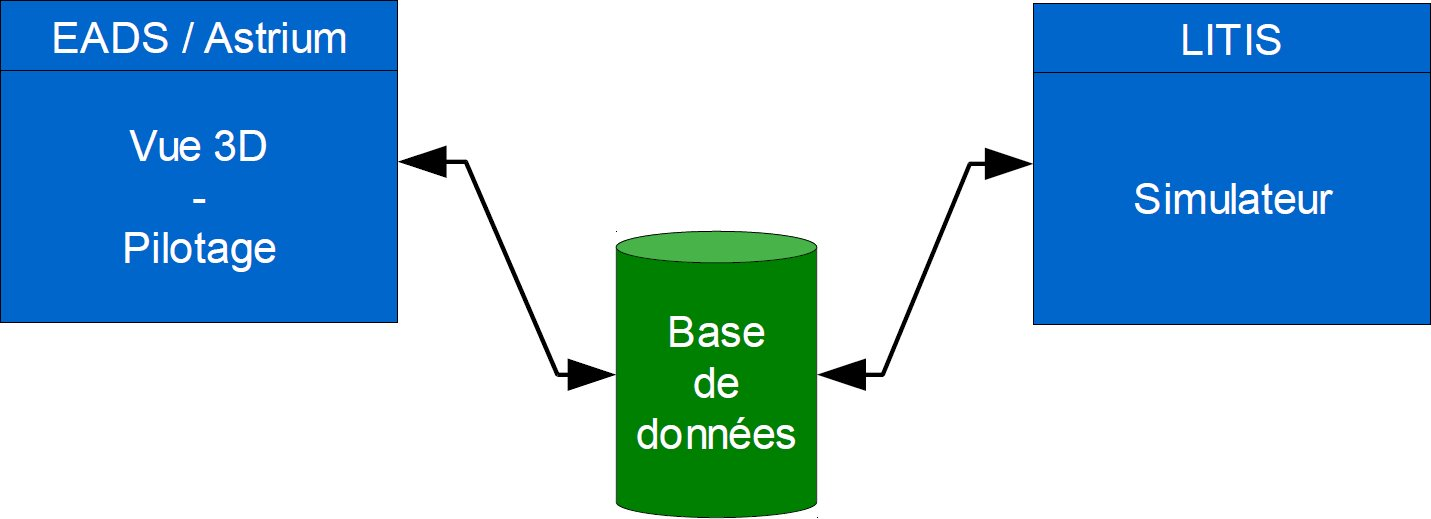
\includegraphics[width=0.75\textwidth]{chapitres/simulation/comEADSLITIS.jpg}
\caption{Communications entre la vue 3D et le simulateur}
\label{fig:simulation:comEADSLITIS}
\end{figure}

La lecture et l'écriture de données dans la base est réalisée à travers des scripts PHP hébergés sur un serveur web ayant accès à la base puis formate le résultat dans un tableau à l'intérieur d'un fichier \verb!XML!. La figure \ref{fig:simulation:scriptPHP} donne un exemple d'accès en lecture à la base de données.

\begin{figure}[ht]
\begin{lstlisting}[language=PHP,escapeinside={@}{@}]
<?php
  try {
    @\$@host = @\$@_POST['host'];
    @\$@dbName = @\$@_POST['dbName'];
    @\$@user = @\$@_POST['user'];
    @\$@password = @\$@_POST['password'];

    @\$@request = @\$@_POST['request'];
    @\$@request = stripslashes(@\$@request);
    @\$@pdo_options[PDO::ATTR_ERRMODE] = PDO::ERRMODE_EXCEPTION;
    @\$@bdd = new PDO("mysql:host=@\$host@;dbname=@\$dbName@", @\$@user, @\$@password, @\$@pdo_options);
    @\$@reponse = @\$@bdd->query(@\$@request);
?>
<table>
<?php while (@\$@donnees = @\$@reponse->fetch()){ ?>
  <tr>
  <?php
    @\$@i=0;
    while(@\$@i < count(@\$@donnees)-1) {
  ?>
    <td>
      <?php echo @\$@donnees[@\$@i]; @\$@i=@\$@i+1; ?>
    </td>
    <?php } ?>
  </tr>
  <?php } ?>
</table>
<?php
  @\$@reponse->closeCursor();
  }
  catch(Exception @\$@e) {
    die('Erreur : '.@\$@e->getMessage());
  }
?>
\end{lstlisting}
\caption{script PHP réalisant une requête sur la base de données}
\label{fig:simulation:scriptPHP}
\end{figure}

\FloatBarrier


\section{Modules proposés}

Le simulateur développé propose une liste extensible de modules.

\subsection{Module de mobilité des chariots cavaliers}

Les chariots peuvent être soit pilotés par une IA, soit par un pilote grâce à un joystick au travers de l'interface 3D de EADS / Astrium. Concernant la partie manuelle, les actions effectuées par le pilote sont inscrites dans la base de données et sont ensuite lues par le simulateur qui reproduit les actions sur le modèle. Aucune vérification d'applicabilité n'est alors effectué puisque cette action est réalisée dans le programme d'EADS / Astrium.
L'IA développée dans le module automatique permet de reproduire le comportement du véhicule en terme de déplacements et d'opérations. Les déplacements consistent à respecter le réseau routier et les zones de stockage du terminal ainsi que d'éviter les collisions entre les véhicules. À chaque itération du simulateur, un véhicule contrôlé par l'IA calcule sa future position en fonction de sa position courante, de sa destination et de sa vitesse. La direction à prendre lui est donnée par le module de routage.

\subsection{Module de routage des véhicules}

Ce module permet de calculer des plus court chemins entre deux points du terminal. Plusieurs algorithmes sont ainsi implémentés et des interfaces sont proposées afin de permettre d'ajouter facilement d'autres algorithmes.

\subsubsection{Floyd Warshall : All Pair Shortest Path}

Cet algorithme calcule une seule fois tous les plus court chemins et sauvegarde les résultats pour que leur récupération soit rapide. La complexité est en $O(n^ 3)$ et le temps d'exécution peut donc être assez long.
Cet algorithme est donc inutilisable dans des graphes trop dynamiques.

\subsubsection{Dijkstra}

Cet algorithme calcule les plus court chemins entre un sommet et tous les autres sommets du graphe. Avec un graphe de m arcs et n n\oe{}uds la complexité est de $O[(m+n)*ln(n)]$.

\subsubsection{A * (A Star)}

Il calcule un plus court chemin entre deux sommets du graphe grâce à une heuristique. C'est un algorithme très rapide mais la qualité de la solution ainsi que sa vitesse d'obtention dépend de l'adaptation de l'heuristique à la topologie du graphe. La complexité de cet algorithme dépend également de l'heuristique utilisée. 
Une seule heuristique a été pour le moment implémentée et réalise une estimation du temps de parcours entre deux sommets en calculant le ratio entre la distance (heuristique de Manhattan) et la vitesse du chariot.

\subsubsection{Dijkstra avec prise en compte des temps d'attente en entrée de travée}

Cet algorithme calcule les plus court chemins en temps entre un sommet et tous les autres sommets du graphe avec prise en compte des blocages dans les travées (arcs FIFO) (voir \ref{chap:contexte:opt:routageVehicules} p\pageref{chap:contexte:opt:routageVehicules}) grâce à un mécanisme de réservation de chemins. La complexité de cet algorithme est semblable à celle de Dijkstra.

\subsection{Module d'ordonnancement des missions}

Ce module permet de calculer l'ordonnancement des missions à réaliser sur le terminal. Les missions sont placées dans un pool de tâches à exécuter par les chariots cavaliers. Ces derniers représentent donc des ressources. Le calcul doit tenir compte des fenêtres de temps des missions afin de proposer une solution acceptable pour les clients du terminal (navires, trains ou camions).

\begin{figure}[h]
\centering
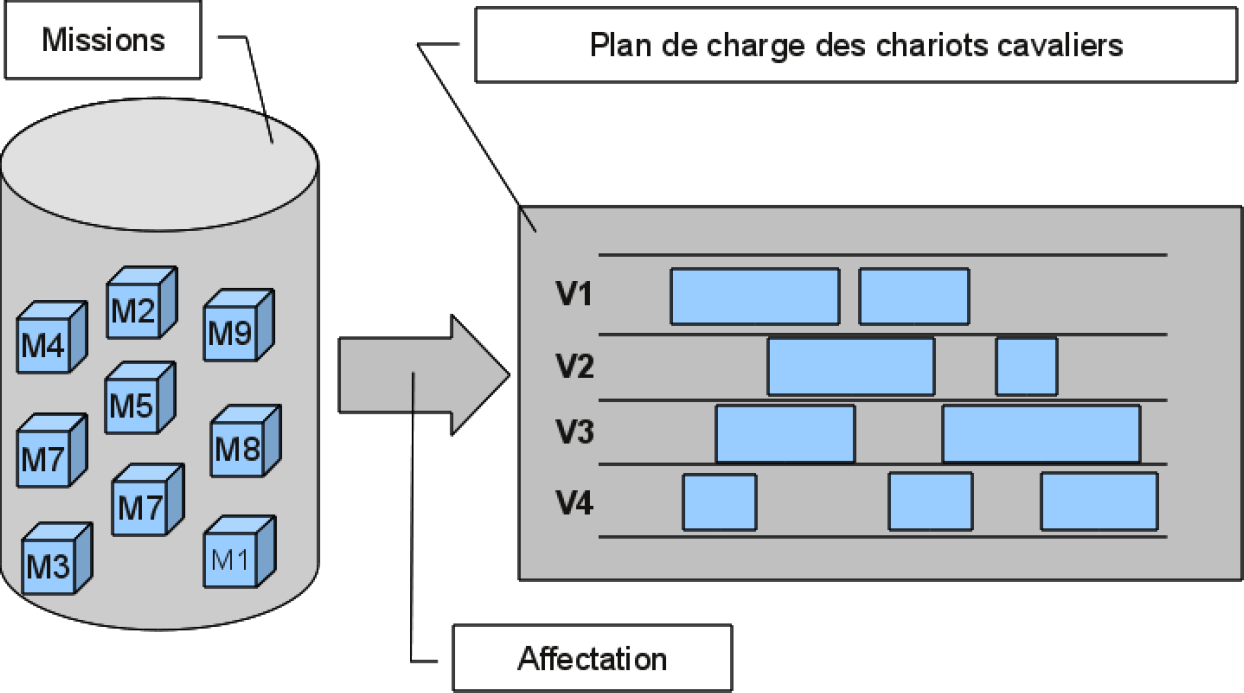
\includegraphics[width=0.75\textwidth]{chapitres/simulation/ordonnancement.png}
\caption{Affectation des missions aux chariots cavaliers}
 \label{fig:simulation:ordonnancement}
\end{figure}

Dans le soucis de réduire les coûts d'exploitation du terminal ainsi que de maintenir une qualité de service suffisante pour les clients, le système doit prendre en compte plusieurs paramètres lors de l'affectation des missions de chargement/déchargement aux chariots cavaliers. Ainsi, la distance à effectuer et le temps de parcours lié à une mission va avoir un impact direct sur le coût de la mission pour le chariot cavalier (consommation de carburant, temps occupé) ainsi que sur le respect des fenêtres de temps pour le client. En effet, si le chariot cavalier arrive trop tard sur le lieu de collecte ou de livraison, le client devra l'attendre. Cette attente a un coût et le client peut réclamer des indemnités au terminal. En revanche, si le chariot cavalier arrive en avance sur le lieu de collecte/livraison, alors il devra attendre le client devenant ainsi indisponible pour d'autres tâches dans le même temps. Plusieurs algorithmes sont développés afin de répondre à ces problématiques. Ils peuvent être 
statiques ou dynamiques. Les algorithmes statiques sont performants mais demandent de recalculer entièrement une solution dès qu'une mission est insérée ou supprimée ou qu'une ressource devient indisponible. En revanche, les algorithmes dynamiques proposent des solutions ``acceptables'' à tout moment.

Chaque algorithme d'ordonnancement et d'affectation présenté dans le chapitre \ref{chapitre:ordo} a été implémenté dans le simulateur. Le module d'ordonnancement contient donc les algorithmes décris dans le tableau suivant : 

% \begin{center}
%  \footnotesize
% \begin{tabular}{|p{7.9cm} p{2.75cm}| p{3.8cm}|}
% 
%   \hline 
%  \multicolumn{2}{|c|}{\textbf{Algorithme}} & \multicolumn{1}{c|}{\textbf{rmiBindingName}} \tabularnewline \hline
%  Branch-and-Bound & (voir \ref{chap:ordo:reso:BB} p\pageref{chap:ordo:reso:BB}) & BranchAndBoundScheduler \tabularnewline \hline
%  Aléatoire & (voir \ref{chap:ordo:reso:random} p\pageref{chap:ordo:reso:random}) & RandomScheduler \tabularnewline \hline
%  Répartition de charge & (voir \ref{chap:ordo:reso:linear} p\pageref{chap:ordo:reso:linear}) & LinearScheduler \tabularnewline \hline
%  Gloutonne : heuristique des plus proches voisins & (voir \ref{chap:ordo:sec:resolution:subsec:heuristiques:glouton} p\pageref{chap:ordo:sec:resolution:subsec:heuristiques:glouton}) & GreedyScheduler \tabularnewline \hline
%  Gloutonne élaborée & (voir \ref{chap:ordo:reso:greedyOpt} p\pageref{chap:ordo:reso:greedyOpt}) & GreedyOptScheduler \tabularnewline \hline
%  Métaheuristique fourmi hors-ligne & (voir \ref{chap:ordo:reso:offlineACO} p\pageref{chap:ordo:reso:offlineACO}) & OfflineACOScheduler \tabularnewline \hline
%  Métaheuristique fourmi en-ligne & (voir \ref{chap:ordo:reso:onlineACO} p\pageref{chap:ordo:reso:onlineACO}) & OnlineACOScheduler \tabularnewline \hline
% \end{tabular}
% \end{center}

\begin{center}
 \footnotesize
\begin{tabular}{|p{10cm}| p{3.8cm}|}
 \hline 
 \multicolumn{1}{|c|}{\textbf{Algorithme}} & \multicolumn{1}{c|}{\textbf{rmiBindingName}} \tabularnewline \hline
 Branch-and-Bound (voir \ref{chap:ordo:reso:BB} p\pageref{chap:ordo:reso:BB}) & BranchAndBoundScheduler \tabularnewline \hline
 Aléatoire (voir \ref{chap:ordo:reso:random} p\pageref{chap:ordo:reso:random}) & RandomScheduler \tabularnewline \hline
 Répartition de charge (voir \ref{chap:ordo:reso:linear} p\pageref{chap:ordo:reso:linear}) & LinearScheduler \tabularnewline \hline
 Gloutonne : heuristique des plus proches voisins (voir \ref{chap:ordo:sec:resolution:subsec:heuristiques:glouton} p\pageref{chap:ordo:sec:resolution:subsec:heuristiques:glouton}) & GreedyScheduler \tabularnewline \hline
 Gloutonne élaborée (voir \ref{chap:ordo:reso:greedyOpt} p\pageref{chap:ordo:reso:greedyOpt}) & GreedyOptScheduler \tabularnewline \hline
 Métaheuristique fourmi hors-ligne (voir \ref{chap:ordo:reso:offlineACO} p\pageref{chap:ordo:reso:offlineACO}) & OfflineACOScheduler \tabularnewline \hline
 Variante de la métaheuristique fourmi hors-ligne (voir \ref{chap:ordo:reso:offlineACO2} p\pageref{chap:ordo:reso:offlineACO2}) & OfflineACOScheduler2 \tabularnewline \hline
 Métaheuristique fourmi en-ligne (voir \ref{chap:ordo:reso:onlineACO} p\pageref{chap:ordo:reso:onlineACO}) & OnlineACOScheduler \tabularnewline \hline
\end{tabular}
\end{center}

\subsection{Module de représentation 2D du terminal}

Ce module permet de visualiser en 2 dimensions l'évolution du terminal. Il contient trois parties :
\begin{itemize}
 \item la vue;
 \item la partie informative;
 \item la partie contrôle;
 \item la partie ordonnancement.
\end{itemize}

\subsubsection{Vue}

La partie vue représente le graphe routier du terminal, le réseau de stockage, les conteneurs et les chariots cavaliers. Cette vue utilise la librairie GraphStream (voir \href{http://graphstream-project.org}{http://graphstream-project.org}) permettant de dessiner entièrement ces éléments de façon très simple grâce à des feuilles de style \verb!CSS!. Le module développé propose un \verb!Listener! sur les modifications du terminal et permet à l'utilisateur de définir des actions en cas d'ajout/suppression de routes ou de conteneurs, de déplacement de véhicule, etc. De cette façon, à tout moment, la vue 2D représente graphiquement et avec exactitude l'état du système.

\subsubsection{Informations}

La partie informative du module de représentation 2D contient des informations sous forme de texte à propos de l'état du terminal. On y trouve des informations sur les missions connues du systèmes (conteneur concerné, destination, fenêtres de temps, état, chariot cavalier affecté...), sur les conteneurs (position), sur les véhicules (position, état, plan de charge) ou sur les travées du terminal (contenu des emplacements). Lorsqu'un élément est sélectionné par l'utilisateur dans cette vue, les éléments de la vue 2D concernés par ces informations sont mis en évidence graphiquement. Cette vue est développée en \verb!JAVA! au travers de la librairie \verb!Swing!.

\subsubsection{Contrôleur}

La partie contrôle concerne le déroulement de la simulation. Elle permet à l'utilisateur de définir le pas de temps, puis de démarrer la simulation. Une fois lancée, il peut également la mettre en pause et avancer itération par itération, relancer la simulation ou quitter le programme. D'autre part, dans le cas où un chariot se trouve dans l'impossibilité de prendre/déposer un conteneur (conteneur bloqué sous un autre, problème d'alignement, problème d'étage, emplacement plein, etc), une boîte de dialogue apparaît et demande à l'utilisateur de régler ce problème. Pour cela, la boîte de dialogue propose des solutions et l'utilisateur n'a plus qu'à faire son choix.

\begin{figure}[h]
\centering
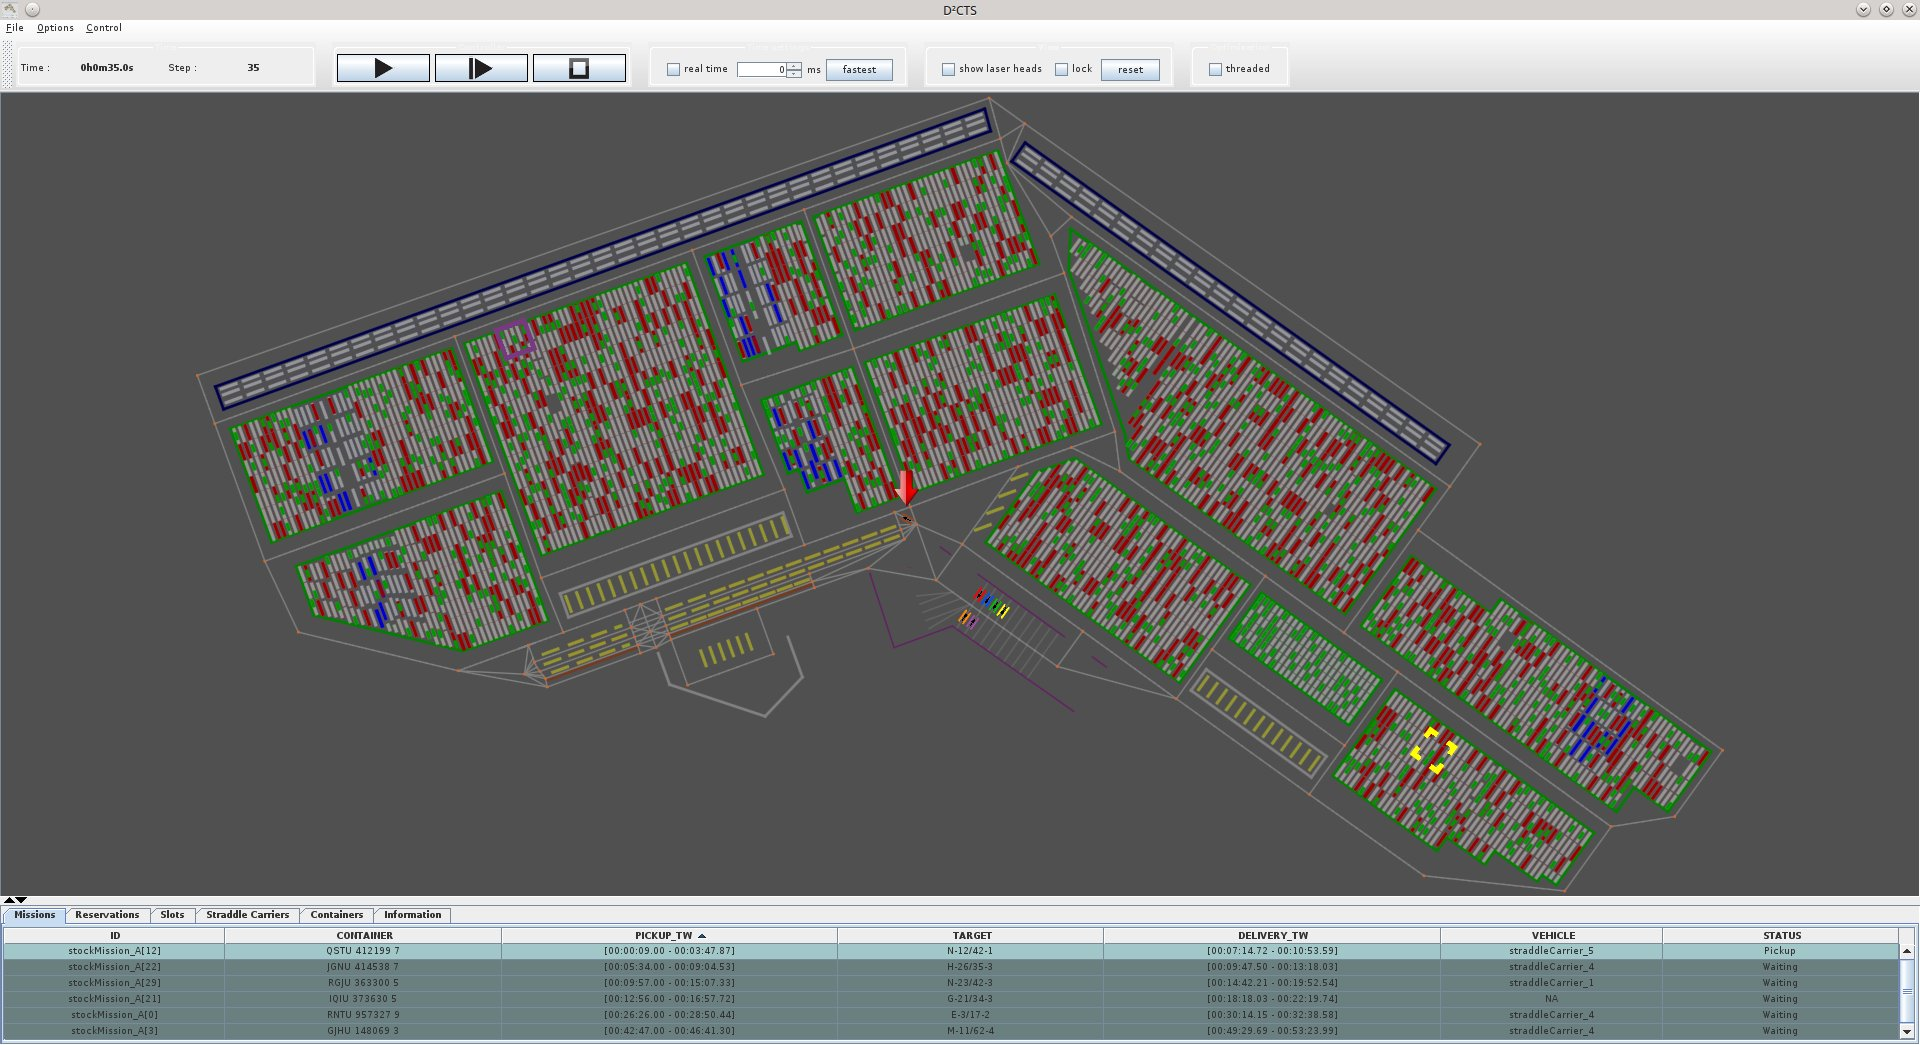
\includegraphics[width=0.85\textwidth]{chapitres/simulation/vue2D-vue-controle-infos.jpg}
\caption{Capture de la partie principale du module graphique du simulateur (en haut le contrôleur, au centre la vue du terminal, en bas la partie informative)}
 \label{fig:simulation:ihm2D}
\end{figure}

\subsubsection{Ordonnanceur}

La partie ordonnancement concerne la performance des affectations des missions aux chariots cavaliers. Selon les critères établis dans le chapitre précédent, cette performance dépend de la distance couverte par les véhicules, du retard lié au dépassement des fenêtres de temps (\textit{tardiness}), ainsi que de la durée d'attente des véhicules aux points de collecte et de livraison (\textit{earliness}). Lorsque l'algorithme de résolution le défini, des données supplémentaires peuvent être affichées, comme le graphe de résolution par exemple pour la méthode de résolution en-ligne utilisant la métaheuristique fourmi.

\begin{figure}[h]
 \centering
 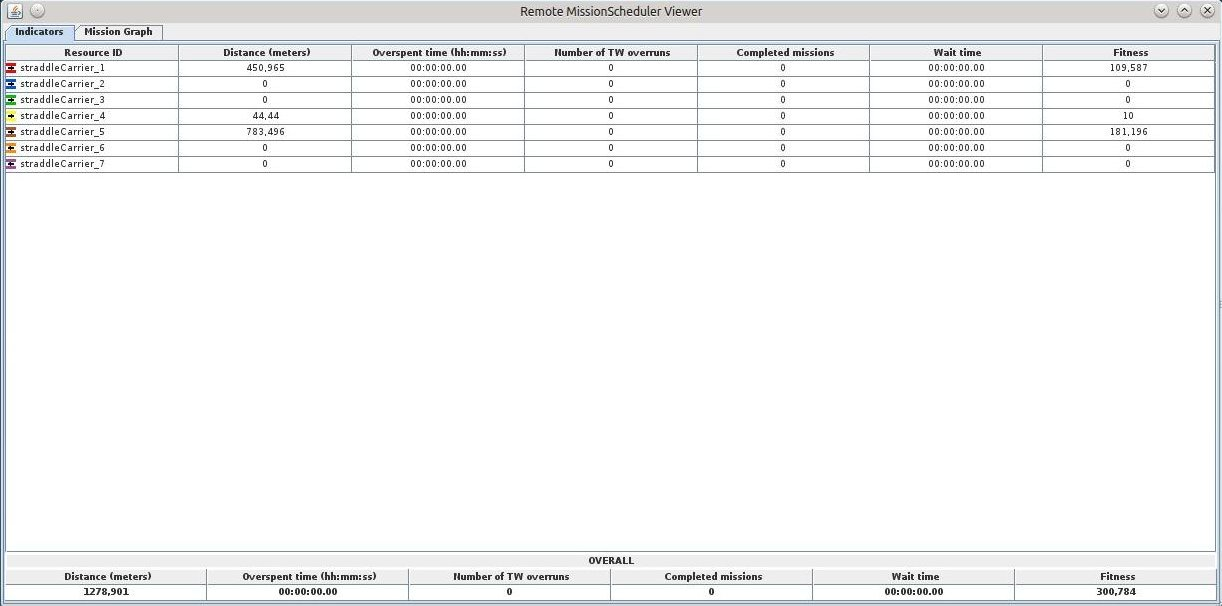
\includegraphics[width=0.85\textwidth]{chapitres/simulation/ordo2D-Infos.jpg}
 \caption{Partie ordonnancement du module graphique du simulateur : informations sur la performance de l'algorithme}
 \label{fig:simulation:ordonnancement2D}
\end{figure}

\begin{figure}[h]
 \centering
 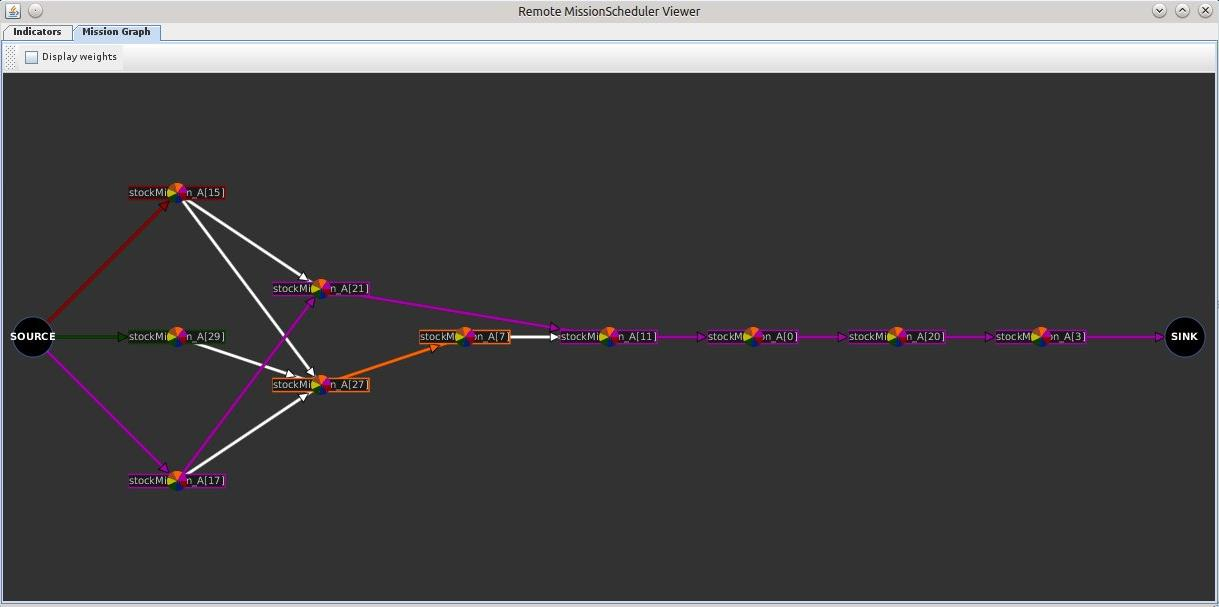
\includegraphics[width=0.85\textwidth]{chapitres/simulation/ordo3D-Graphe.jpg}
 \caption{Partie ordonnancement du module graphique du simulateur : graphe des missions de l'algorithme de résolution en-ligne}
 \label{fig:simulation:ordonnancement2D-2}
\end{figure}

\subsection{Module de transformation XML (\textit{parser})}

Ce module permet de transformer les données \verb!XML! concernant la simulation en informations. Il se compose de 3 parties :
\begin{itemize}
 \item Le \textit{parser} de configuration réseau : transforme les informations décrites dans le fichier de distribution (voir \ref{chap:simulateur:sec:archi:distribution:reseau} p\pageref{chap:simulateur:sec:archi:distribution:reseau});
 \item Le \textit{parser} de configuration du terminal : transforme selon le format défini (voir \ref{chap:simulateur:sec:archi:distribution:contenu} p\pageref{chap:simulateur:sec:archi:distribution:contenu}) les éléments \verb!XML! en objets informatiques afin de décrire les composants du terminal ainsi que son contenu;
 \item Le \textit{parser} de communication avec les chariots cavaliers : permet de définir les actions à réaliser par l'IA des chariots cavaliers en fonctions de messages \verb!XML!.
\end{itemize}
C'est dans ce module que sont définies les règles d'écritures des balises. Un modèle différent peut donc être facilement implémenté en redéfinissant ces classes.

\subsection{Modules de génération de données}
Les générateurs proposés sont des modules permettant de générer des fichiers \verb!XML!. Il existe pour le moment 3 générateurs de données :
\begin{itemize}
 \item le générateur d'état initial;
 \item le générateur de missions;
 \item le générateur d'événements.
\end{itemize}

\subsubsection{Générateur d'état initial}

Ce générateur permet de créer des conteneurs et de les répartir entre les différents emplacements de stockage du terminal. Il utilise les fichiers de configuration du terminal afin de définir la structure du terminal et de connaître son contenu. Il charge donc le graphe routier et le réseau de stockage avant de commencer à générer les conteneurs. La génération se fait selon différents paramètres. Il faut en effet fournir au générateur le nombre de conteneurs de 20 pieds, de 40 pieds et de 45 pieds à créer. De plus, il faut indiquer le nom de la machine sur laquelle le générateur est lancé ainsi que les fichiers de configuration réseau et de terminal à utiliser. Enfin il faut définir le nom du fichier \verb!XML! à générer.

\subsubsection{Générateur de missions}

Ce générateur permet de créer des missions pour les chariots cavaliers. Une mission consiste à déplacer un conteneur à l'intérieur du terminal. Selon le type de mission à définir, le générateur va créer ou non un véhicule (train, bateau, ou navire). Il détermine également si la mission à créer sera de type \verb!IN! ou \verb!OUT! puis, en fonction du résultat décidera du conteneur à déplacer. Si le conteneur entre dans le terminal (mission de type \verb!IN!) alors il sera créé. Ensuite le générateur défini un emplacement de destination pour la livraison du conteneur. Une fois ces informations déterminées le générateur détermine les fenêtres de temps de la mission ainsi que les fenêtres de temps des véhicules concernés. Pour cela il se base sur le temps moyen de parcours entre le point de collecte et de livraison du conteneur. Les fenêtres de temps sont ensuite décalées selon une marge de tolérance d'écart de temps. Ce paramètre est fourni en entrée de l'algorithme.

\subsubsection{Générateurs d'événements}

Le générateur d'événements permet de générer un fichier \verb!XML! contenant des balises \verb!<event>!\verb!</event>! afin de décrire des perturbations sur le système. Il est possible de générer des pannes sur les véhicules, des non respect d'itinéraires par les conducteurs ou de non respect d'affectation de mission. Il est également possible de générer des variations de portée des bornes lasers. Ces événements sont définis en fonction de taux indiqués en entrée du générateur.


L'objectif final de ces générateurs est de pouvoir les configurer en fonction de lois statistiques. Ainsi, les modules de générations sont composés d'interfaces permettant aux utilisateurs de redéfinir les fonctions de générations selon les besoins.

\section{Perspectives}

Les deux premières années de travail sur le projet CALAS ont consisté à modéliser les composants d'un terminal portuaire ainsi que leur dynamique. Le simulateur informatique de terminal a été élaboré autour de l'informatisation du plan du terminal de Normandie grâce à une longue phase de collecte de données.

Le simulateur développé a été conçu pour mettre à l'épreuve différentes approches d'ordonnancement et de routage pour obtenir des résultats permettant d'évaluer la qualité des diverses solutions. Toutefois, il est possible d'utiliser le simulateur pour concevoir des méthodes de résolution à tous les problèmes d'optimisation liés aux terminaux à conteneurs. Il est ainsi possible de mettre à l'épreuve des approches de résolution des problèmes de : 
\begin{itemize}
 \item la structure du terminal;
 \item l’allocation des berges aux navires;
 \item l’allocation des grues de quai;
 \item les plans de chargement des navires;
 \item le transbordement;
 \item la gestion des conteneurs vides;
 \item la gestion des effectifs;
 \item le stockage (allocation des travées et des blocs) ;
 \item les transferts (quai - stockage, stockage - stockage, stockage - terre);
 \item le routage des véhicules;
 \item l’allocation des engins de manutention.
\end{itemize}

Pour le moment, le simulateur n'a été utilisé que pour modéliser les 2 derniers problèmes, néanmoins il est capable de façon intrinsèque de répondre aux autres problématiques.
